\documentclass[t]{beamer}
\usepackage[utf8x]{inputenc}
\usepackage[ngerman]{babel}
\usepackage[T1]{fontenc}
\usepackage{textcomp}
\usepackage{subfigure}
\usepackage{graphicx}
\usepackage{fancyhdr}
\usepackage{tgpagella}
\usepackage[absolute,overlay]{textpos}
\usepackage{hyperref}
\usepackage{wasysym}
% \MakeAutoQuote{„}{”}

% ohne dieses Paket bekommt Carsten verpixelte Schrifen
\usepackage{lmodern}

\hypersetup{
colorlinks=true,
linkcolor=[rgb]{1, 1, 1}, %
urlcolor=[rgb]{.2, .2, .5} %
%allcolors=[rgb]{0, 0, 0} % schwarz
}

\usetheme{Dresden}

\title{Freie Software \& Freies Wissen Dresden}
\subtitle{Uni-Stick-Ausgabe-Veranstaltung}
\author{\texttt{https://fsfw-dresden.de}}
\date{26. Oktober 2017}


\beamertemplatenavigationsymbolsempty

\addtobeamertemplate{frametitle}{}{%
  \begin{textblock*}{130mm}(.963\textwidth,8.4mm)
    
\includegraphics[width=2.25cm]{img-src/fsfw-logo.pdf}
  \end{textblock*}
}


\setbeamercolor{frametitle}{fg=black}

\synctex=1

% \includeonlyframes{p1}

\begin{document}






\begin{frame}[label=p1]
  \begin{center}%
\vspace*{-1em}

\includegraphics[width=4cm]{img-src/fsfw-logo-with-text}\\
\hspace{1cm}
\structure{\Large Wie verändern wir die Gesellschaft?}
  \end{center}
\end{frame}


%%%%%%%%%%%%%%%%%%%%%%%%%%%%%%%%%%%%%%%%%%%%%%%%%%%%%%%%%%%%%%%%%%%%%%%%%%%%%%%%

\begin{frame}[label=photo]{\usebeamercolor[fg]{structure}\color{fg}Aufklärung}
\pause
\begin{itemize}
\only<1-2>{
 \item[Kant:] "`... Ausgang des Menschen aus seiner selbstverschuldeten Unmündigkeit."'
 }
\only<3->{
 \item[FSFW:] "`... Bewahrung der Studierenden vor ihrer selbstverschuldeten Abhängigkeit."'
 }
\end{itemize}
\pause
\smallskip
\begin{center}
 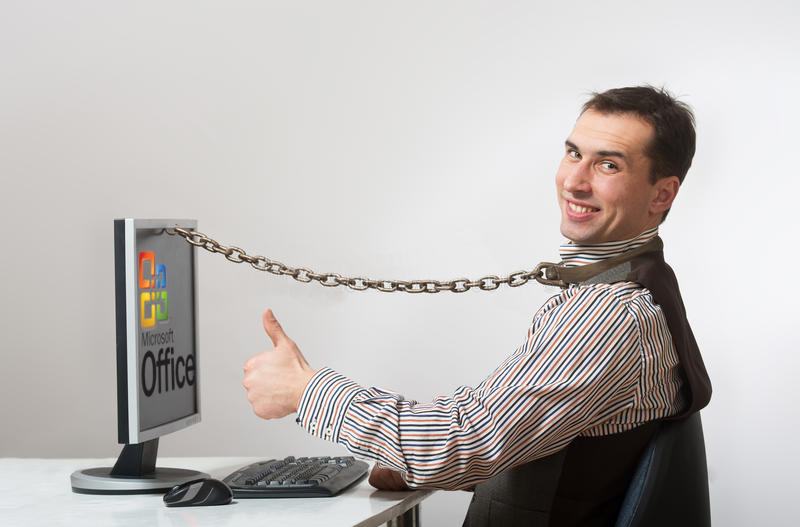
\includegraphics[width=9cm]{img-src/ms-abhaengig}\\[1mm]
\end{center}

 

\end{frame}


%%%%%%%%%%%%%%%%%%%%%%%%%%%%%%%%%%%%%%%%%%%%%%%%%%%%%%%%%%%%%%%%%%%%%%%%%%%%%%%%

% \begin{frame}[label=ct1]{\usebeamercolor[fg]{structure}\color{fg}FSFW (1)}
% Wer sind wir?
%   \begin{itemize}
%   \item Hochschulgruppe (gegründet 2014, ca. 10 P.)
%   \item bisherige Projekte:
%   \begin{itemize}
%    \item Linux-Install-Party, Linux-Presentation-Day
%    \item Verschlüsselungsgewinnspiel
%    \item Monatliche \href{https://fsfw-dresden.de/sprechstunde}{Sprechstunde} (Textsatzsystem \LaTeX, ...)
%    \item Formulierung eines \href{https://fsfw-dresden.de/programm}{Programmpapiers}
%    \item Workshops (\href{https://fsfw-dresden.de/git-ws}{git}, \href{https://fsfw-dresden.de/gpg}{Mailverschlüsselung})
%    \item Uni-Stick mit freier Software
%   \end{itemize}
%   \end{itemize}
% \end{frame}

%%%%%%%%%%%%%%%%%%%%%%%%%%%%%%%%%%%%%%%%%%%%%%%%%%%%%%%%%%%%%%%%%%%%%%%%%%%%%%%%

% \begin{frame}[label=ct2]{\usebeamercolor[fg]{structure}\color{fg}FSFW (2)}
% Warum machen wir das? $\rightarrow$ \textbf{Aus Überzeugung}\\[1cm]
%   \begin{itemize}
%   \item Überzeugung 1: frei und quelloffene Software ist (meist) besser
%   \item[] technische/nicht technische Argumente
%   \pause
%   \bigskip
%   \item Überzeugung 2: \textit{öffentlich finanzierte} wissenschaftliche Inhalte
%   (AutorInnen, GutachterInnen) sollten nicht von \textit{öffentlich finanzierten}
%   Bibliotheken für \textit{horrende Summen} von Zeitschriften-Verlagen gekauft werden müssen
%   \end{itemize}
% \end{frame}


%%%%%%%%%%%%%%%%%%%%%%%%%%%%%%%%%%%%%%%%%%%%%%%%%%%%%%%%%%%%%%%%%%%%%%%%%%%%%%%%
\begin{frame}[label=wb0]{\usebeamercolor[fg]{structure}\color{fg} Vier (Un)Freiheiten}

\only<1>{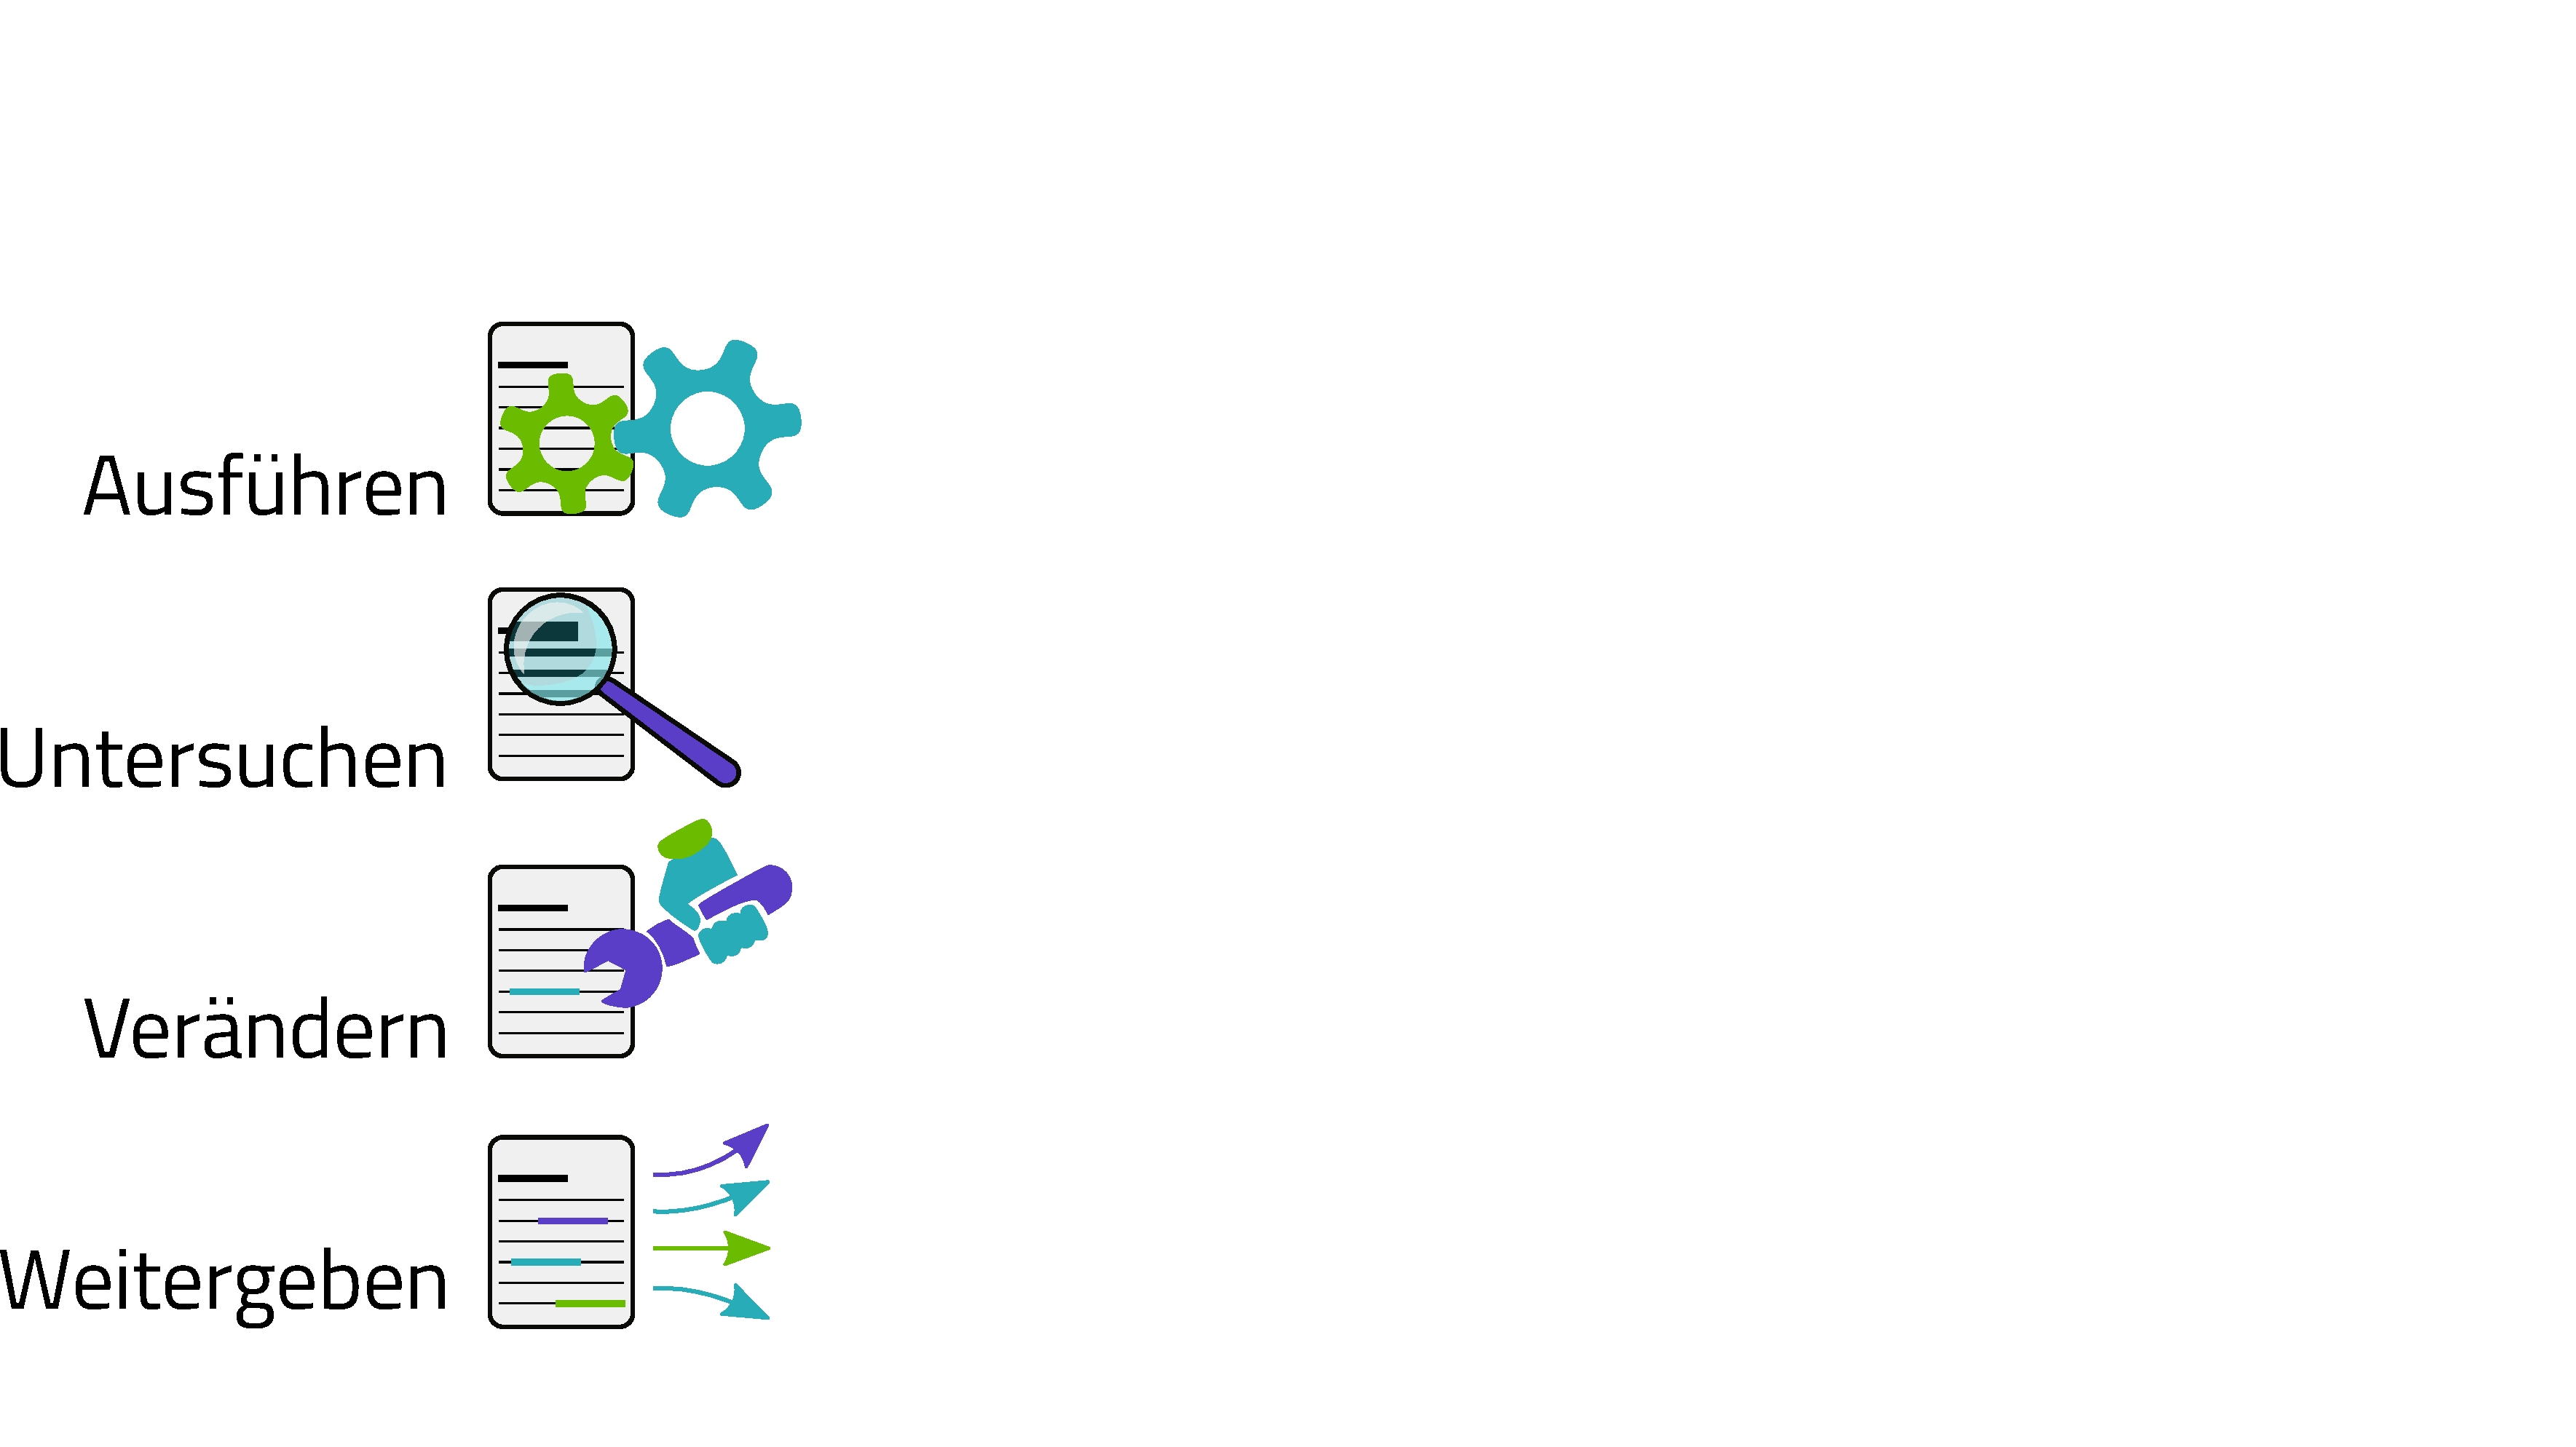
\includegraphics[width=\textwidth]{img-src/vier-freiheiten-tabelle01}}
\only<2>{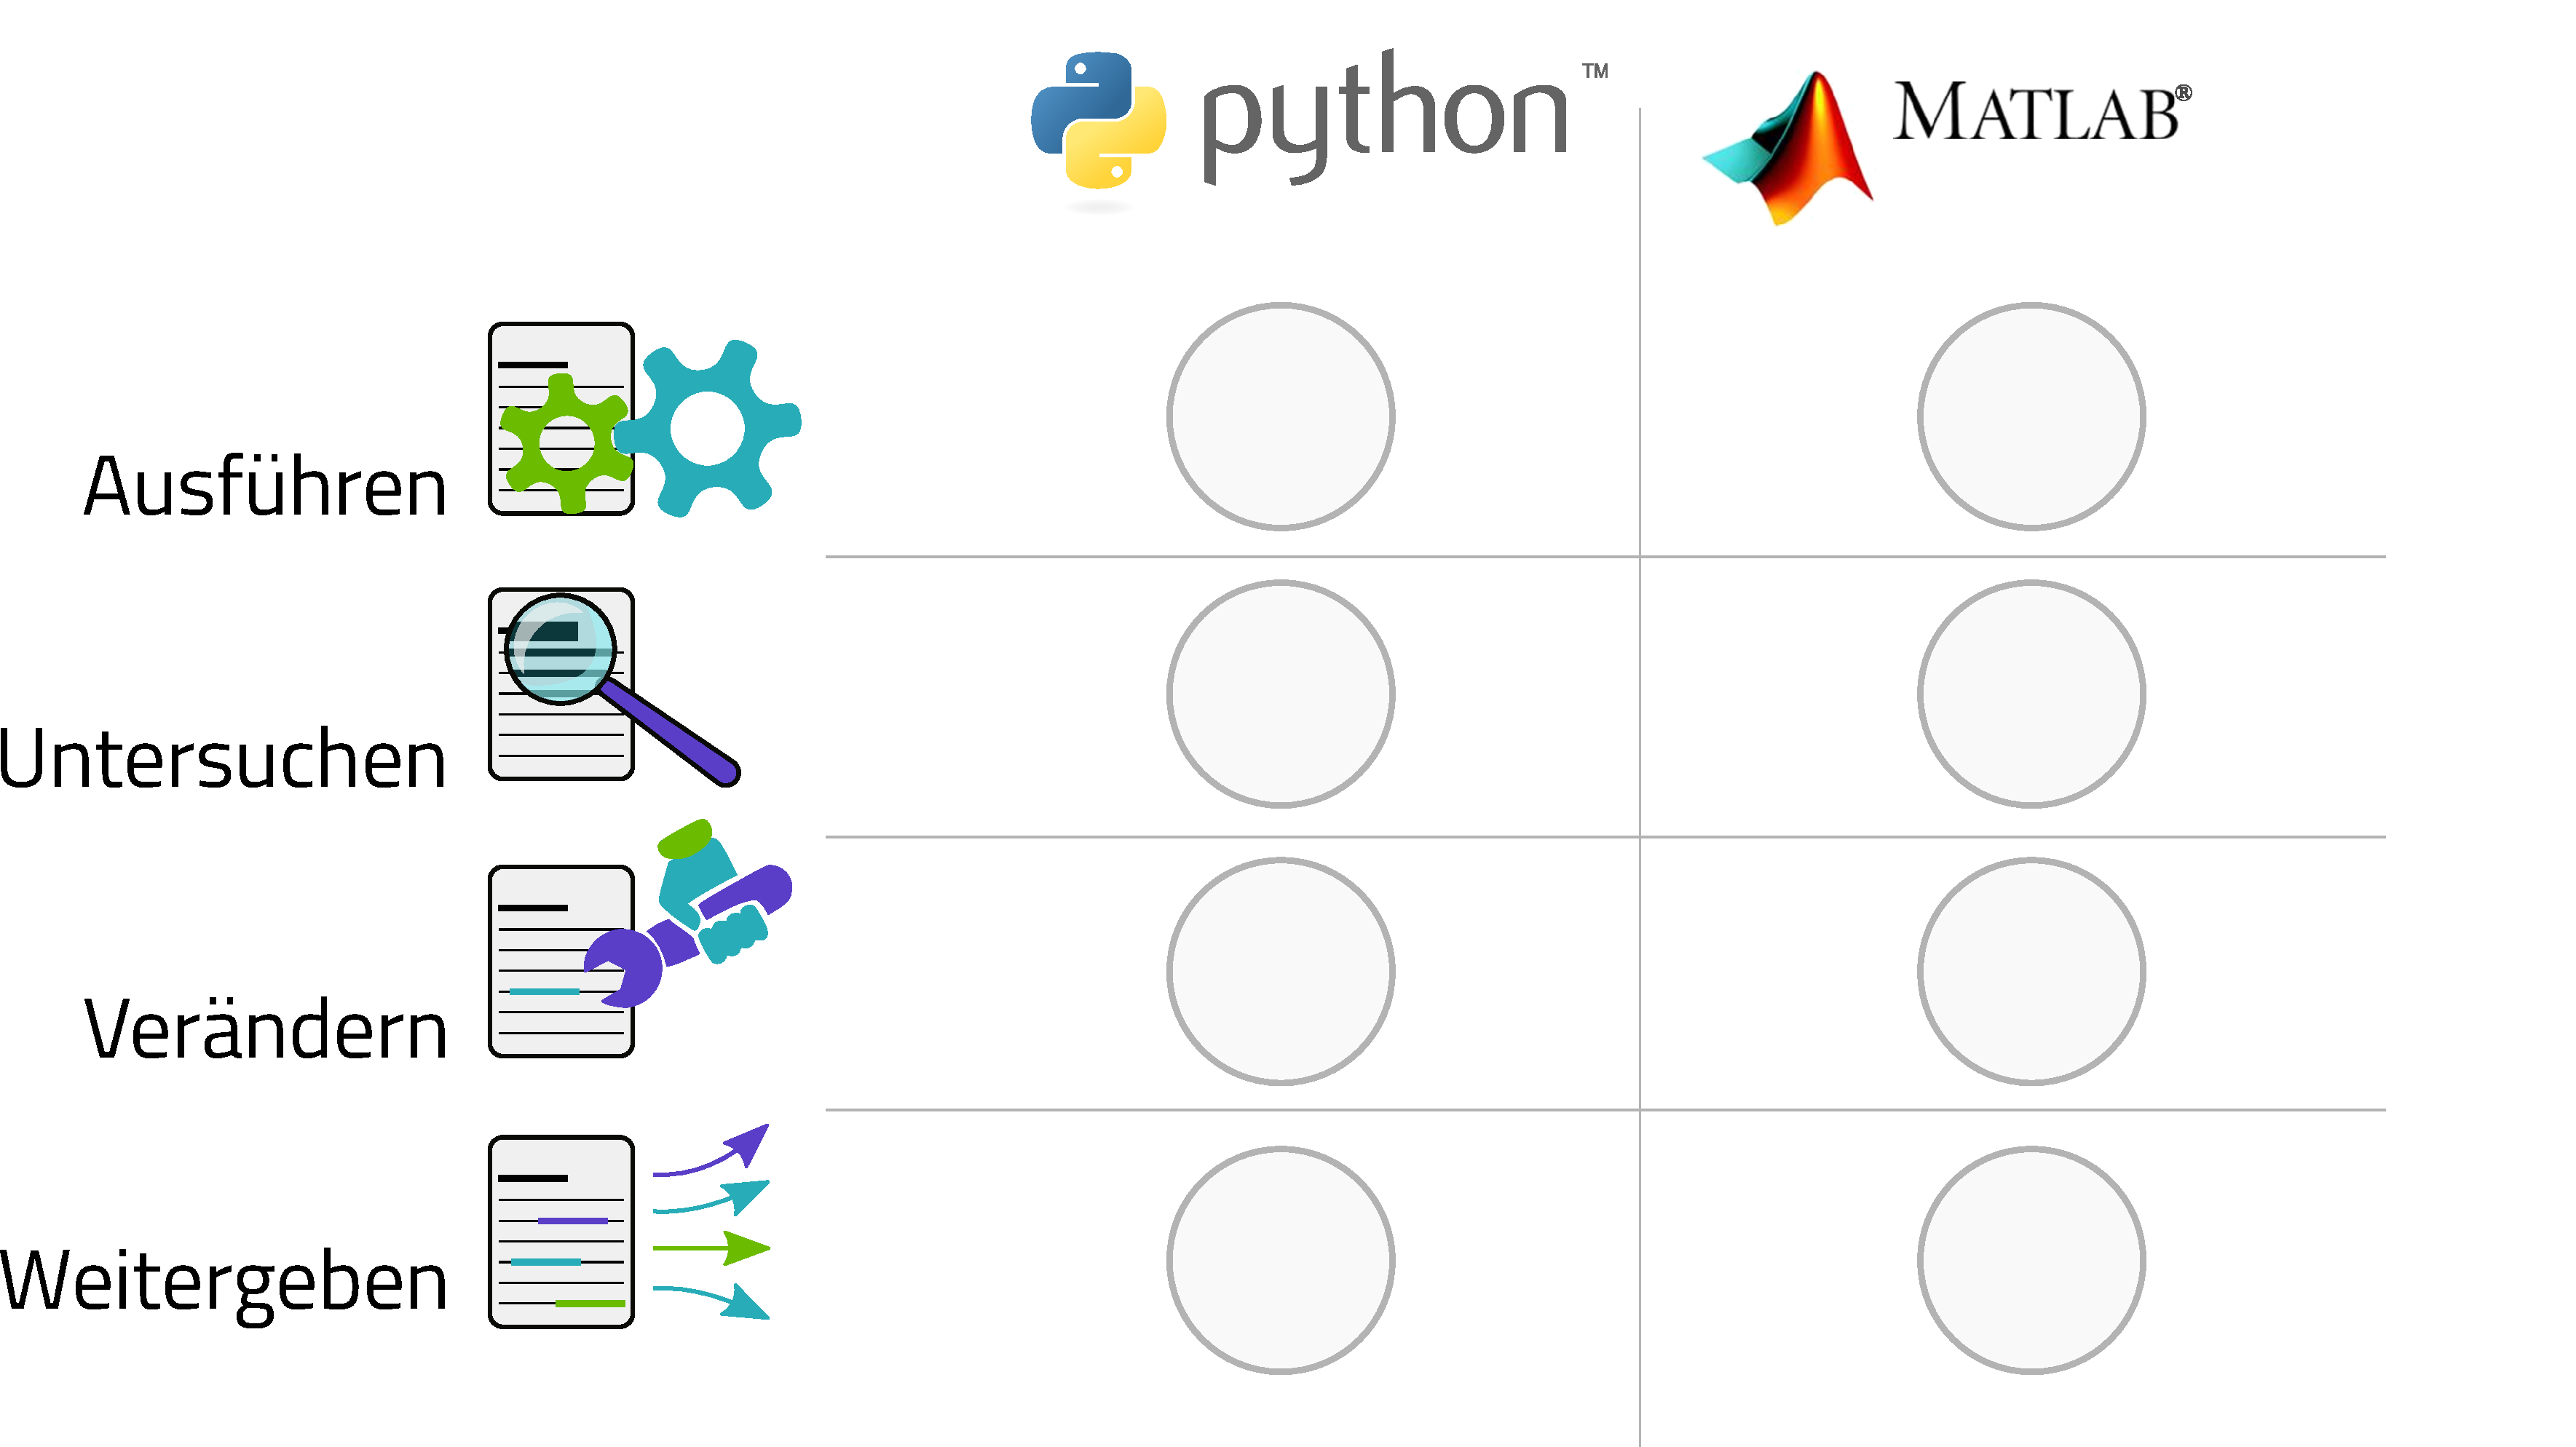
\includegraphics[width=\textwidth]{img-src/vier-freiheiten-tabelle02}}
\only<3>{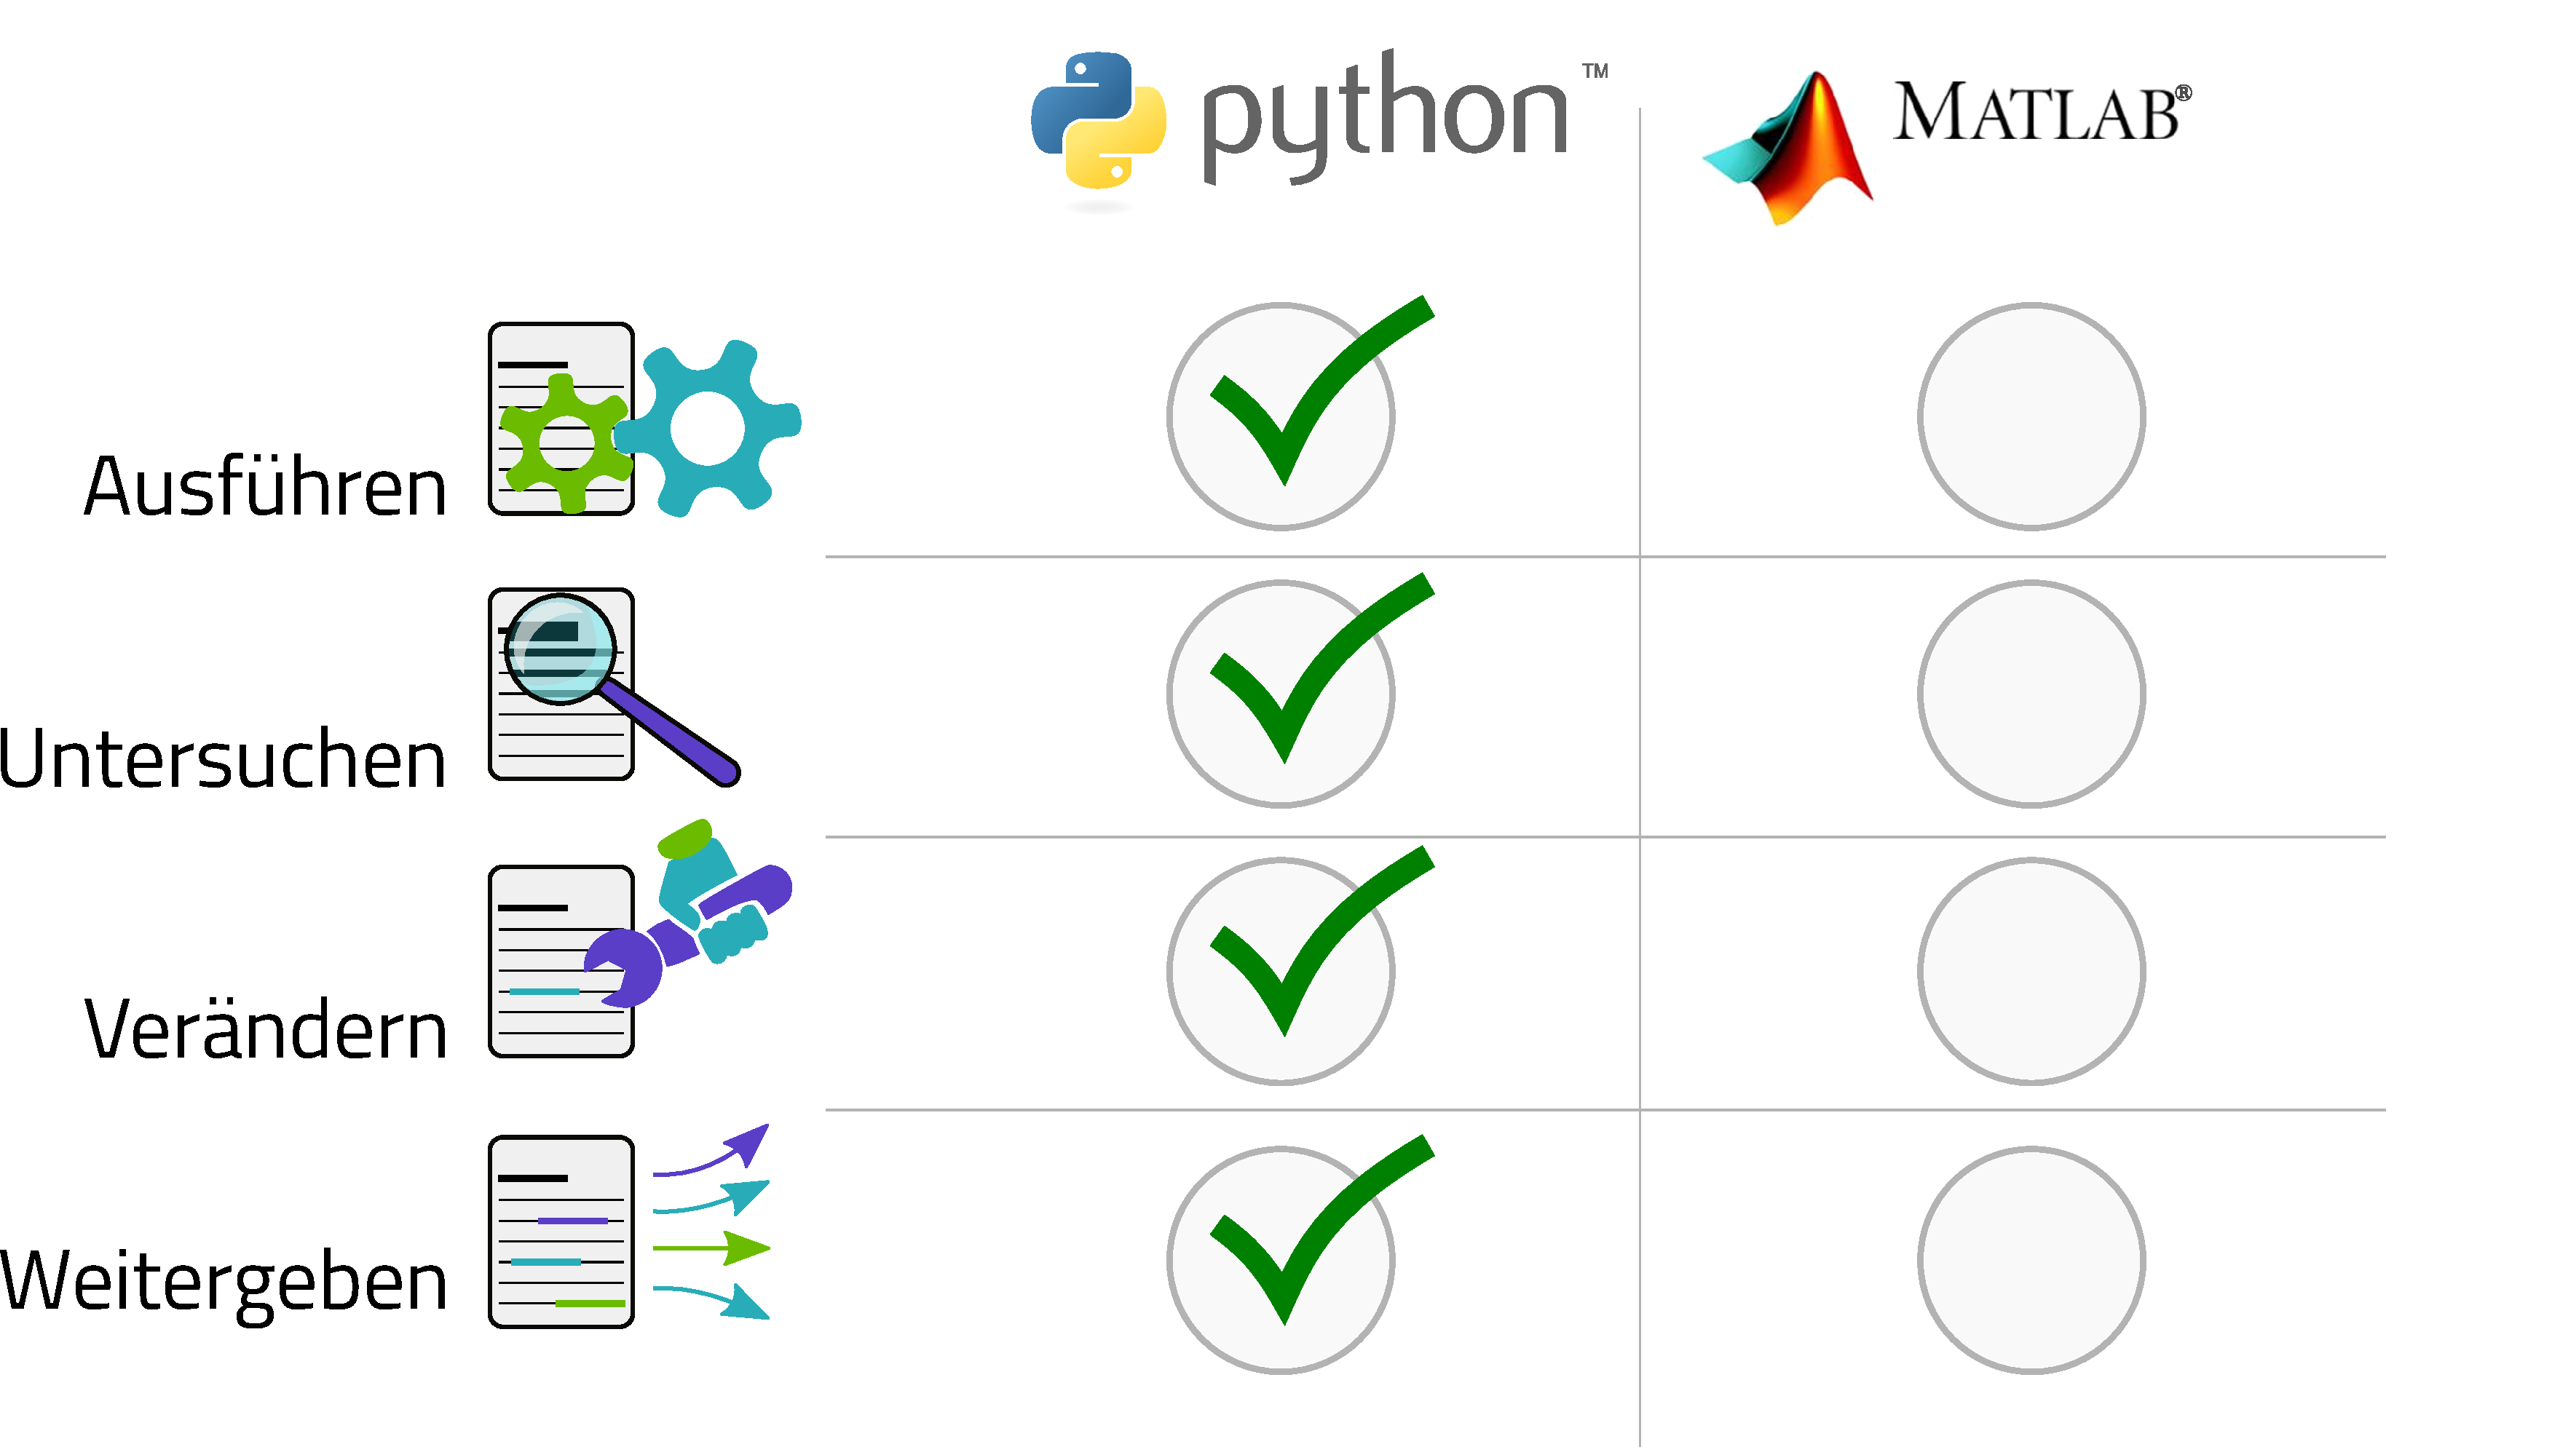
\includegraphics[width=\textwidth]{img-src/vier-freiheiten-tabelle03}}
\only<4>{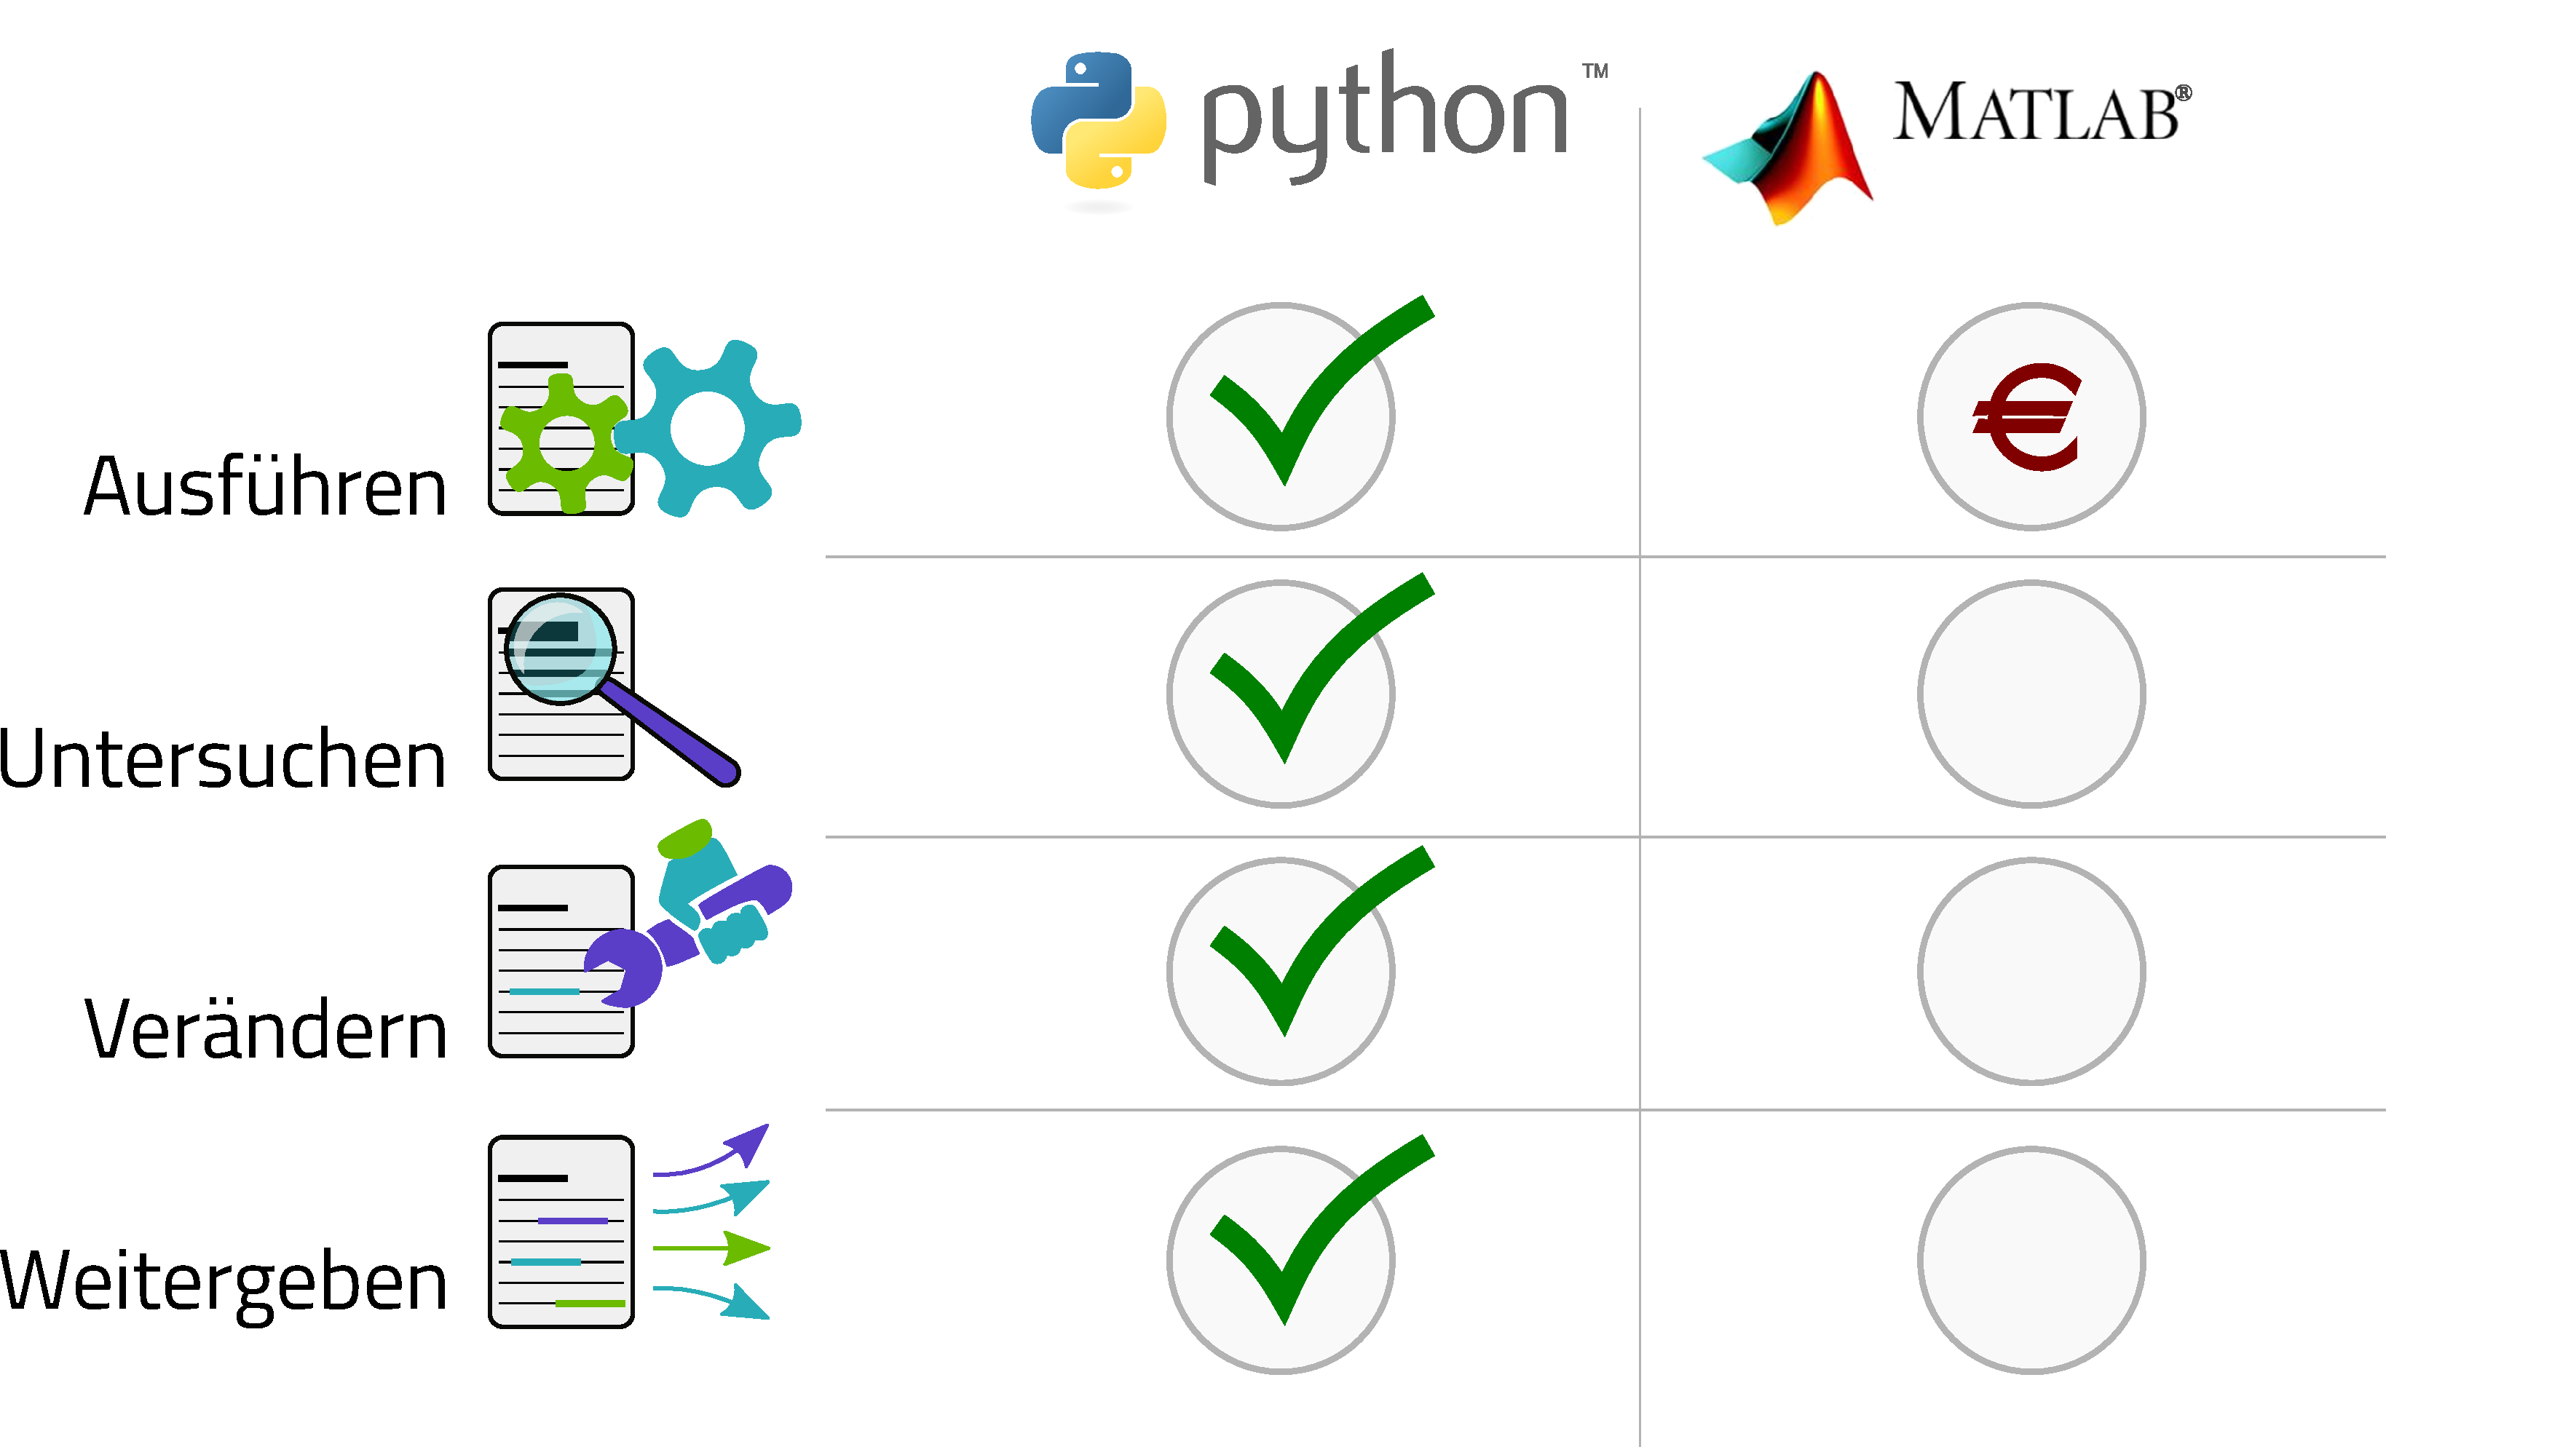
\includegraphics[width=\textwidth]{img-src/vier-freiheiten-tabelle04}}
\only<5>{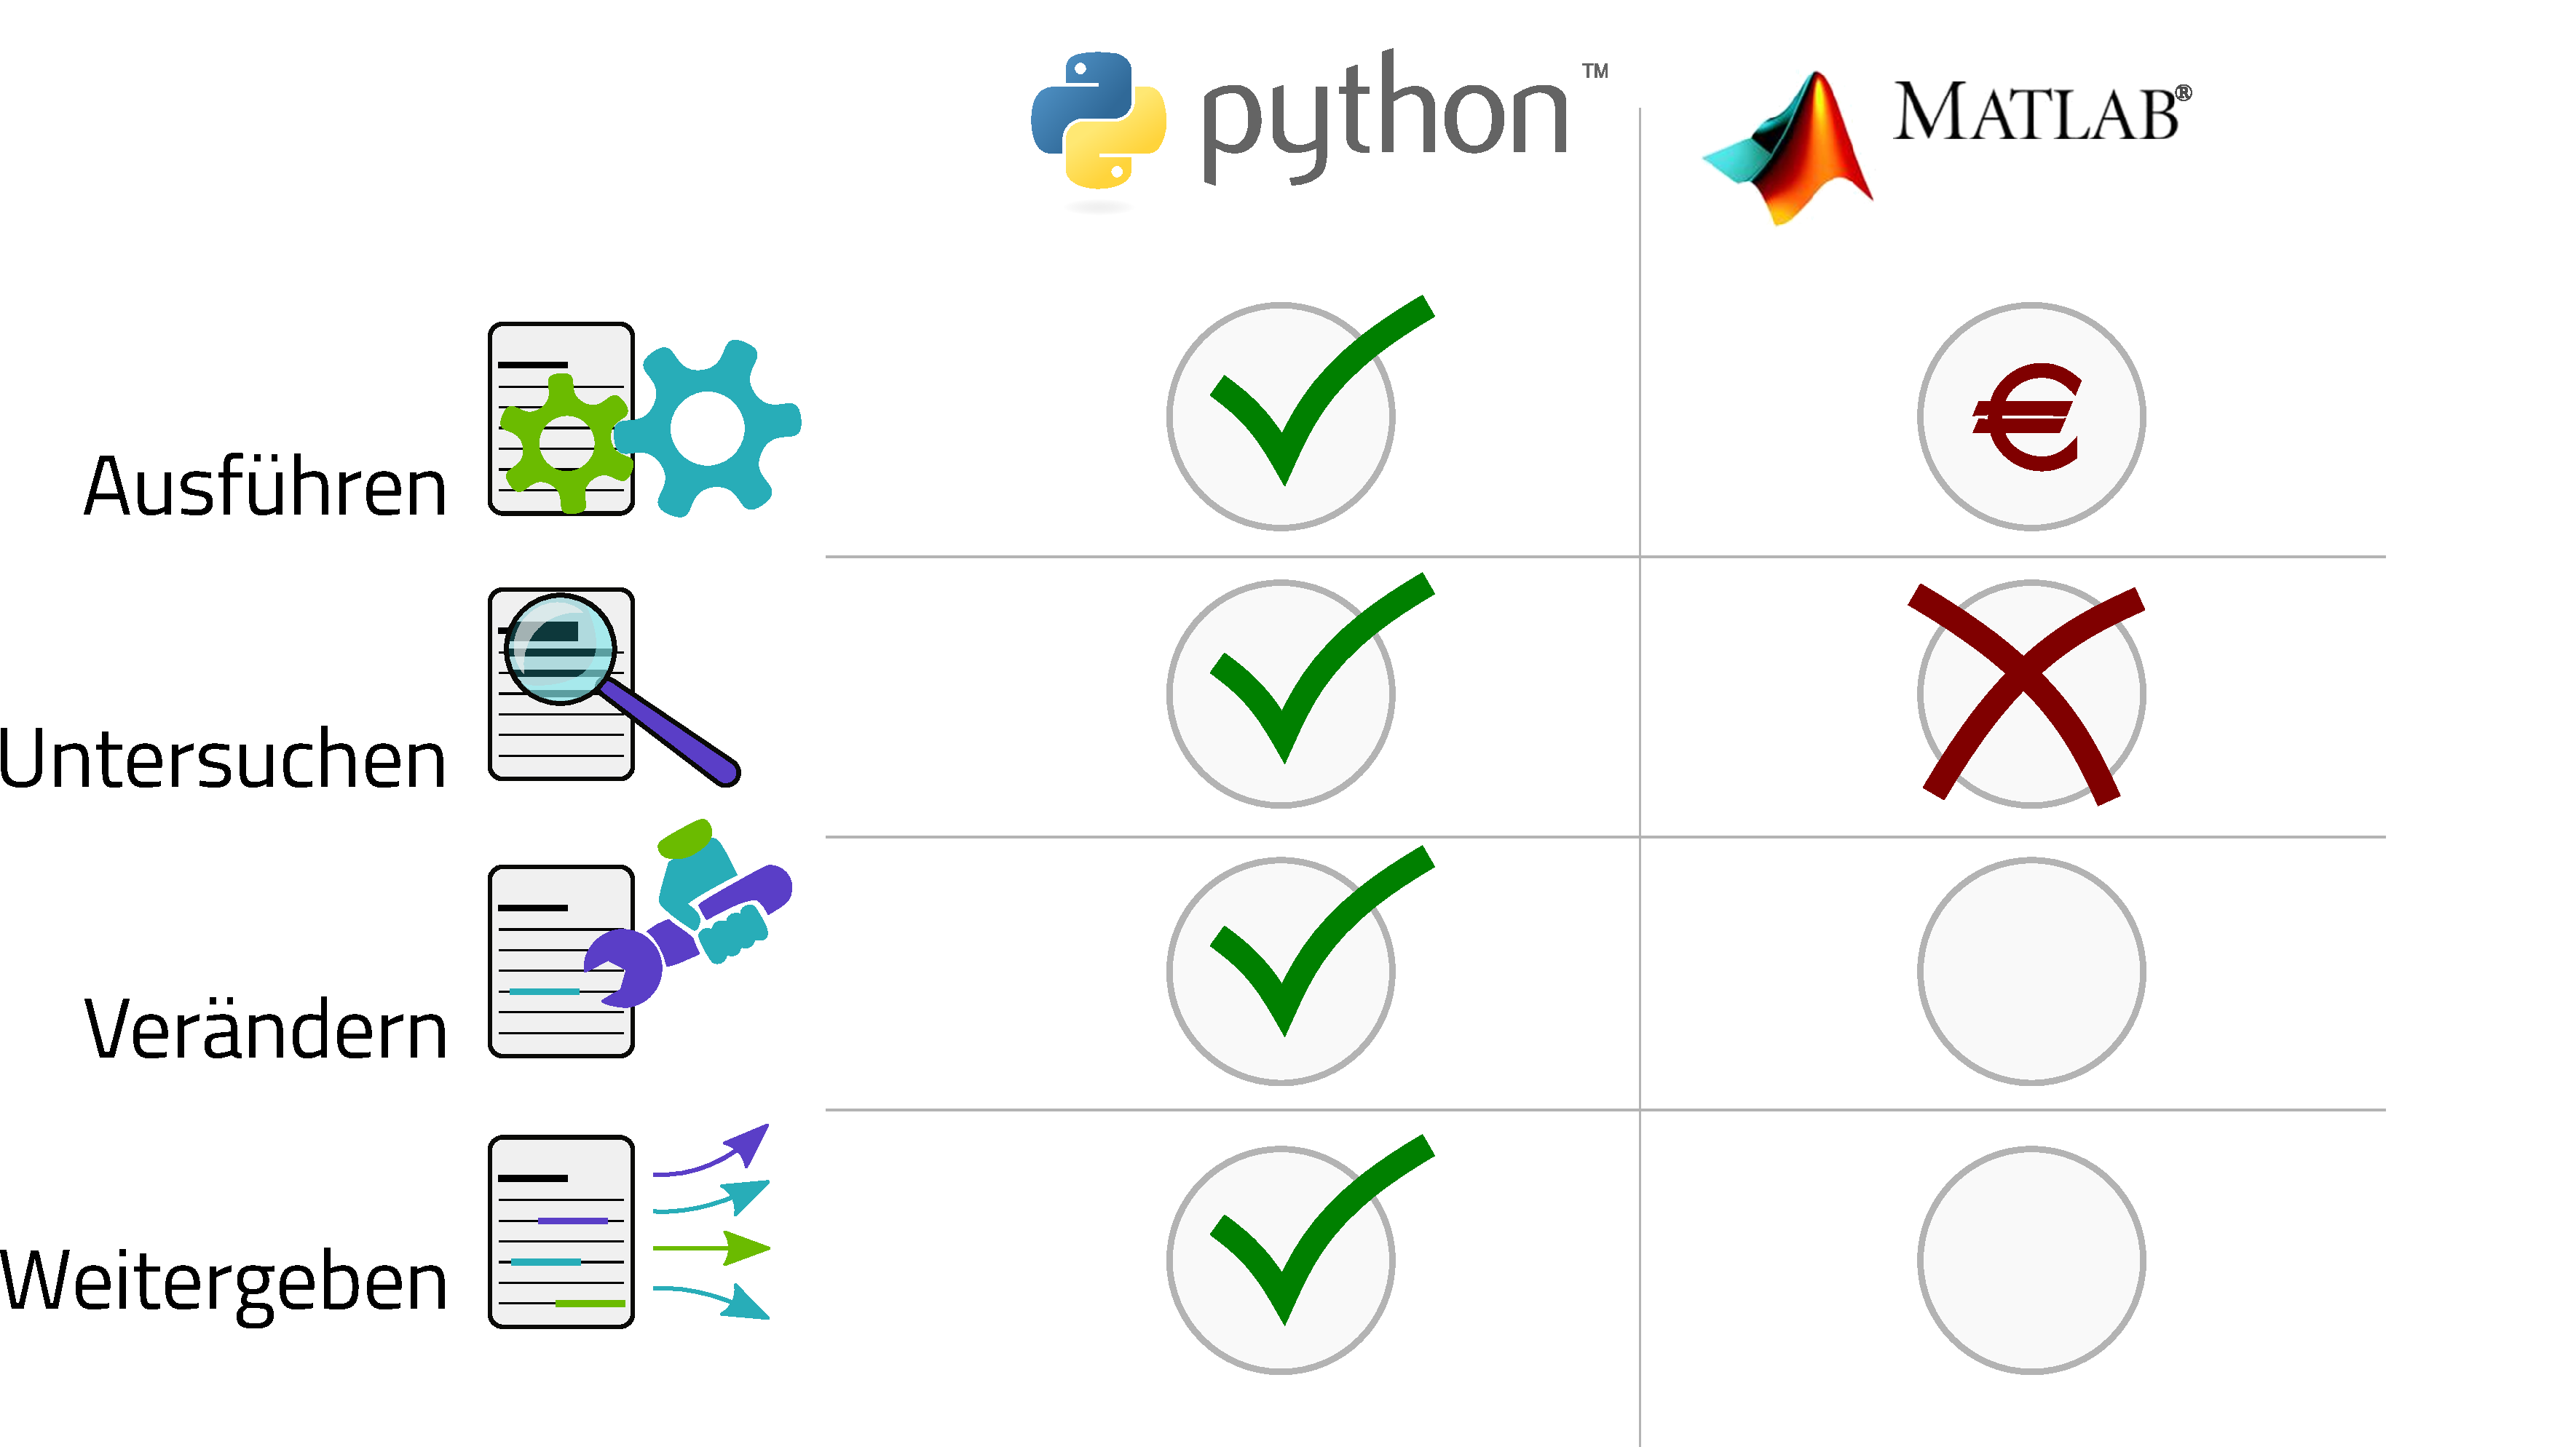
\includegraphics[width=\textwidth]{img-src/vier-freiheiten-tabelle05}}
\only<6>{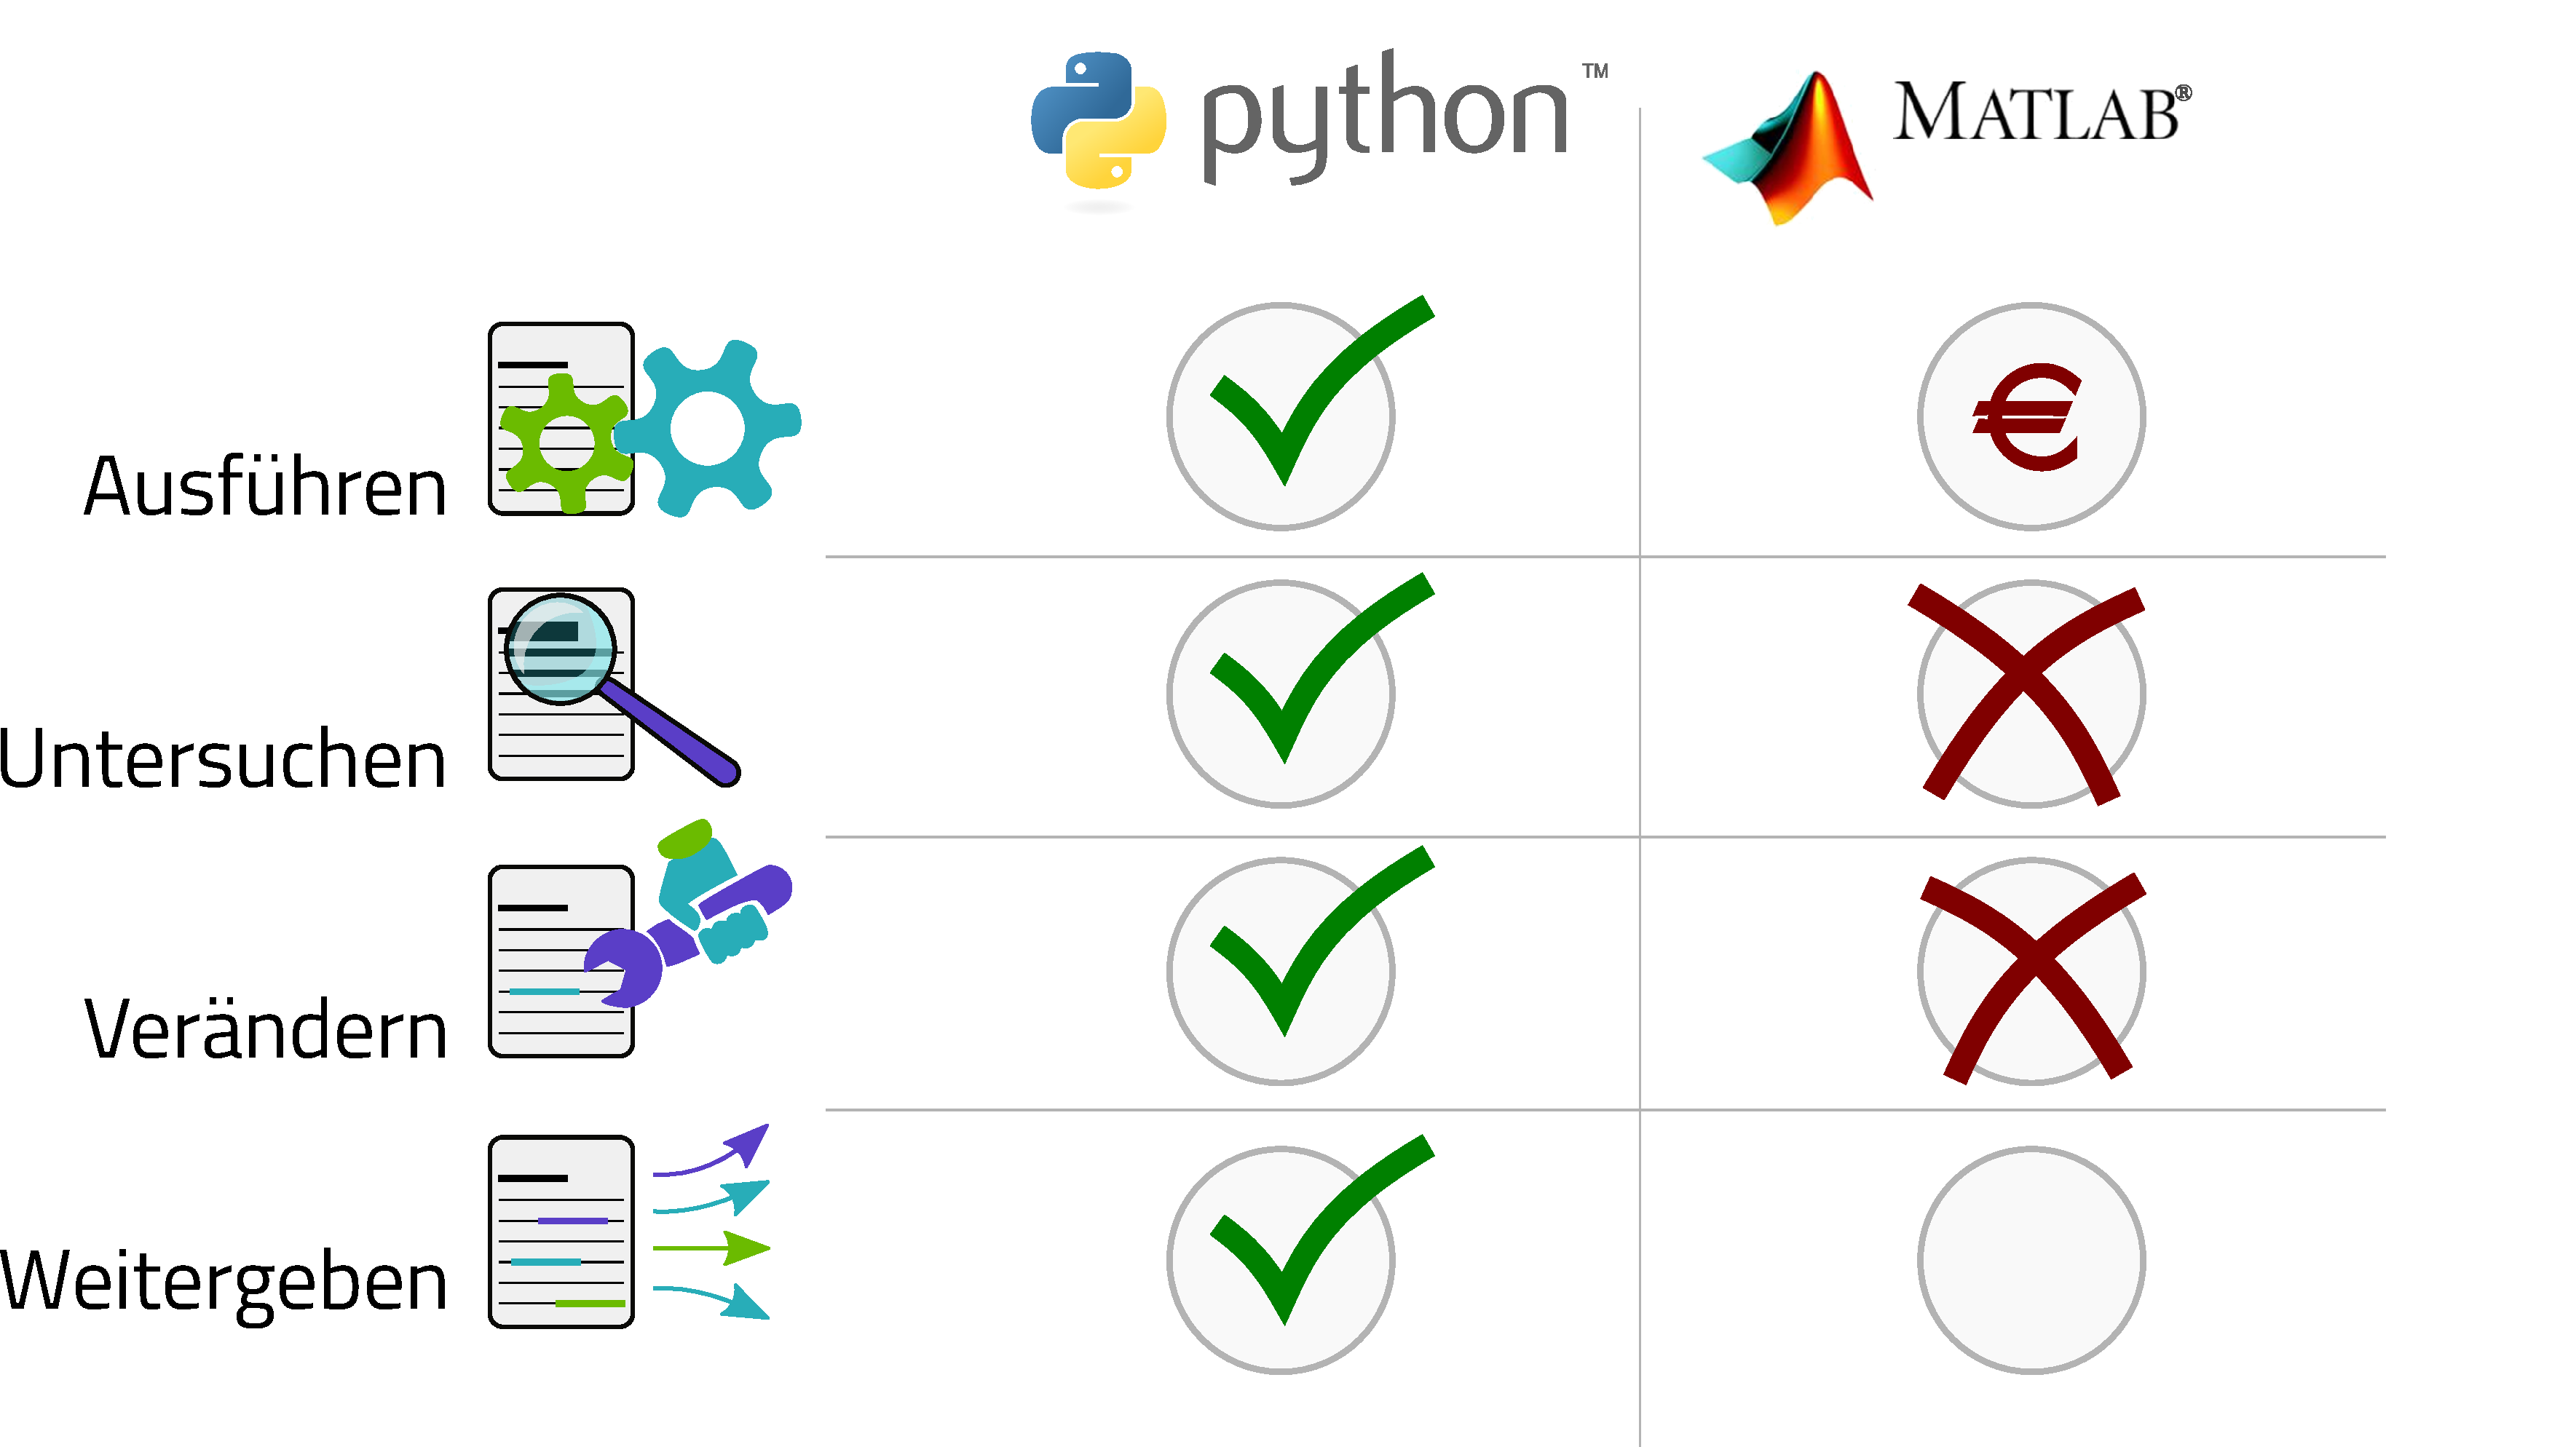
\includegraphics[width=\textwidth]{img-src/vier-freiheiten-tabelle06}}
\only<7>{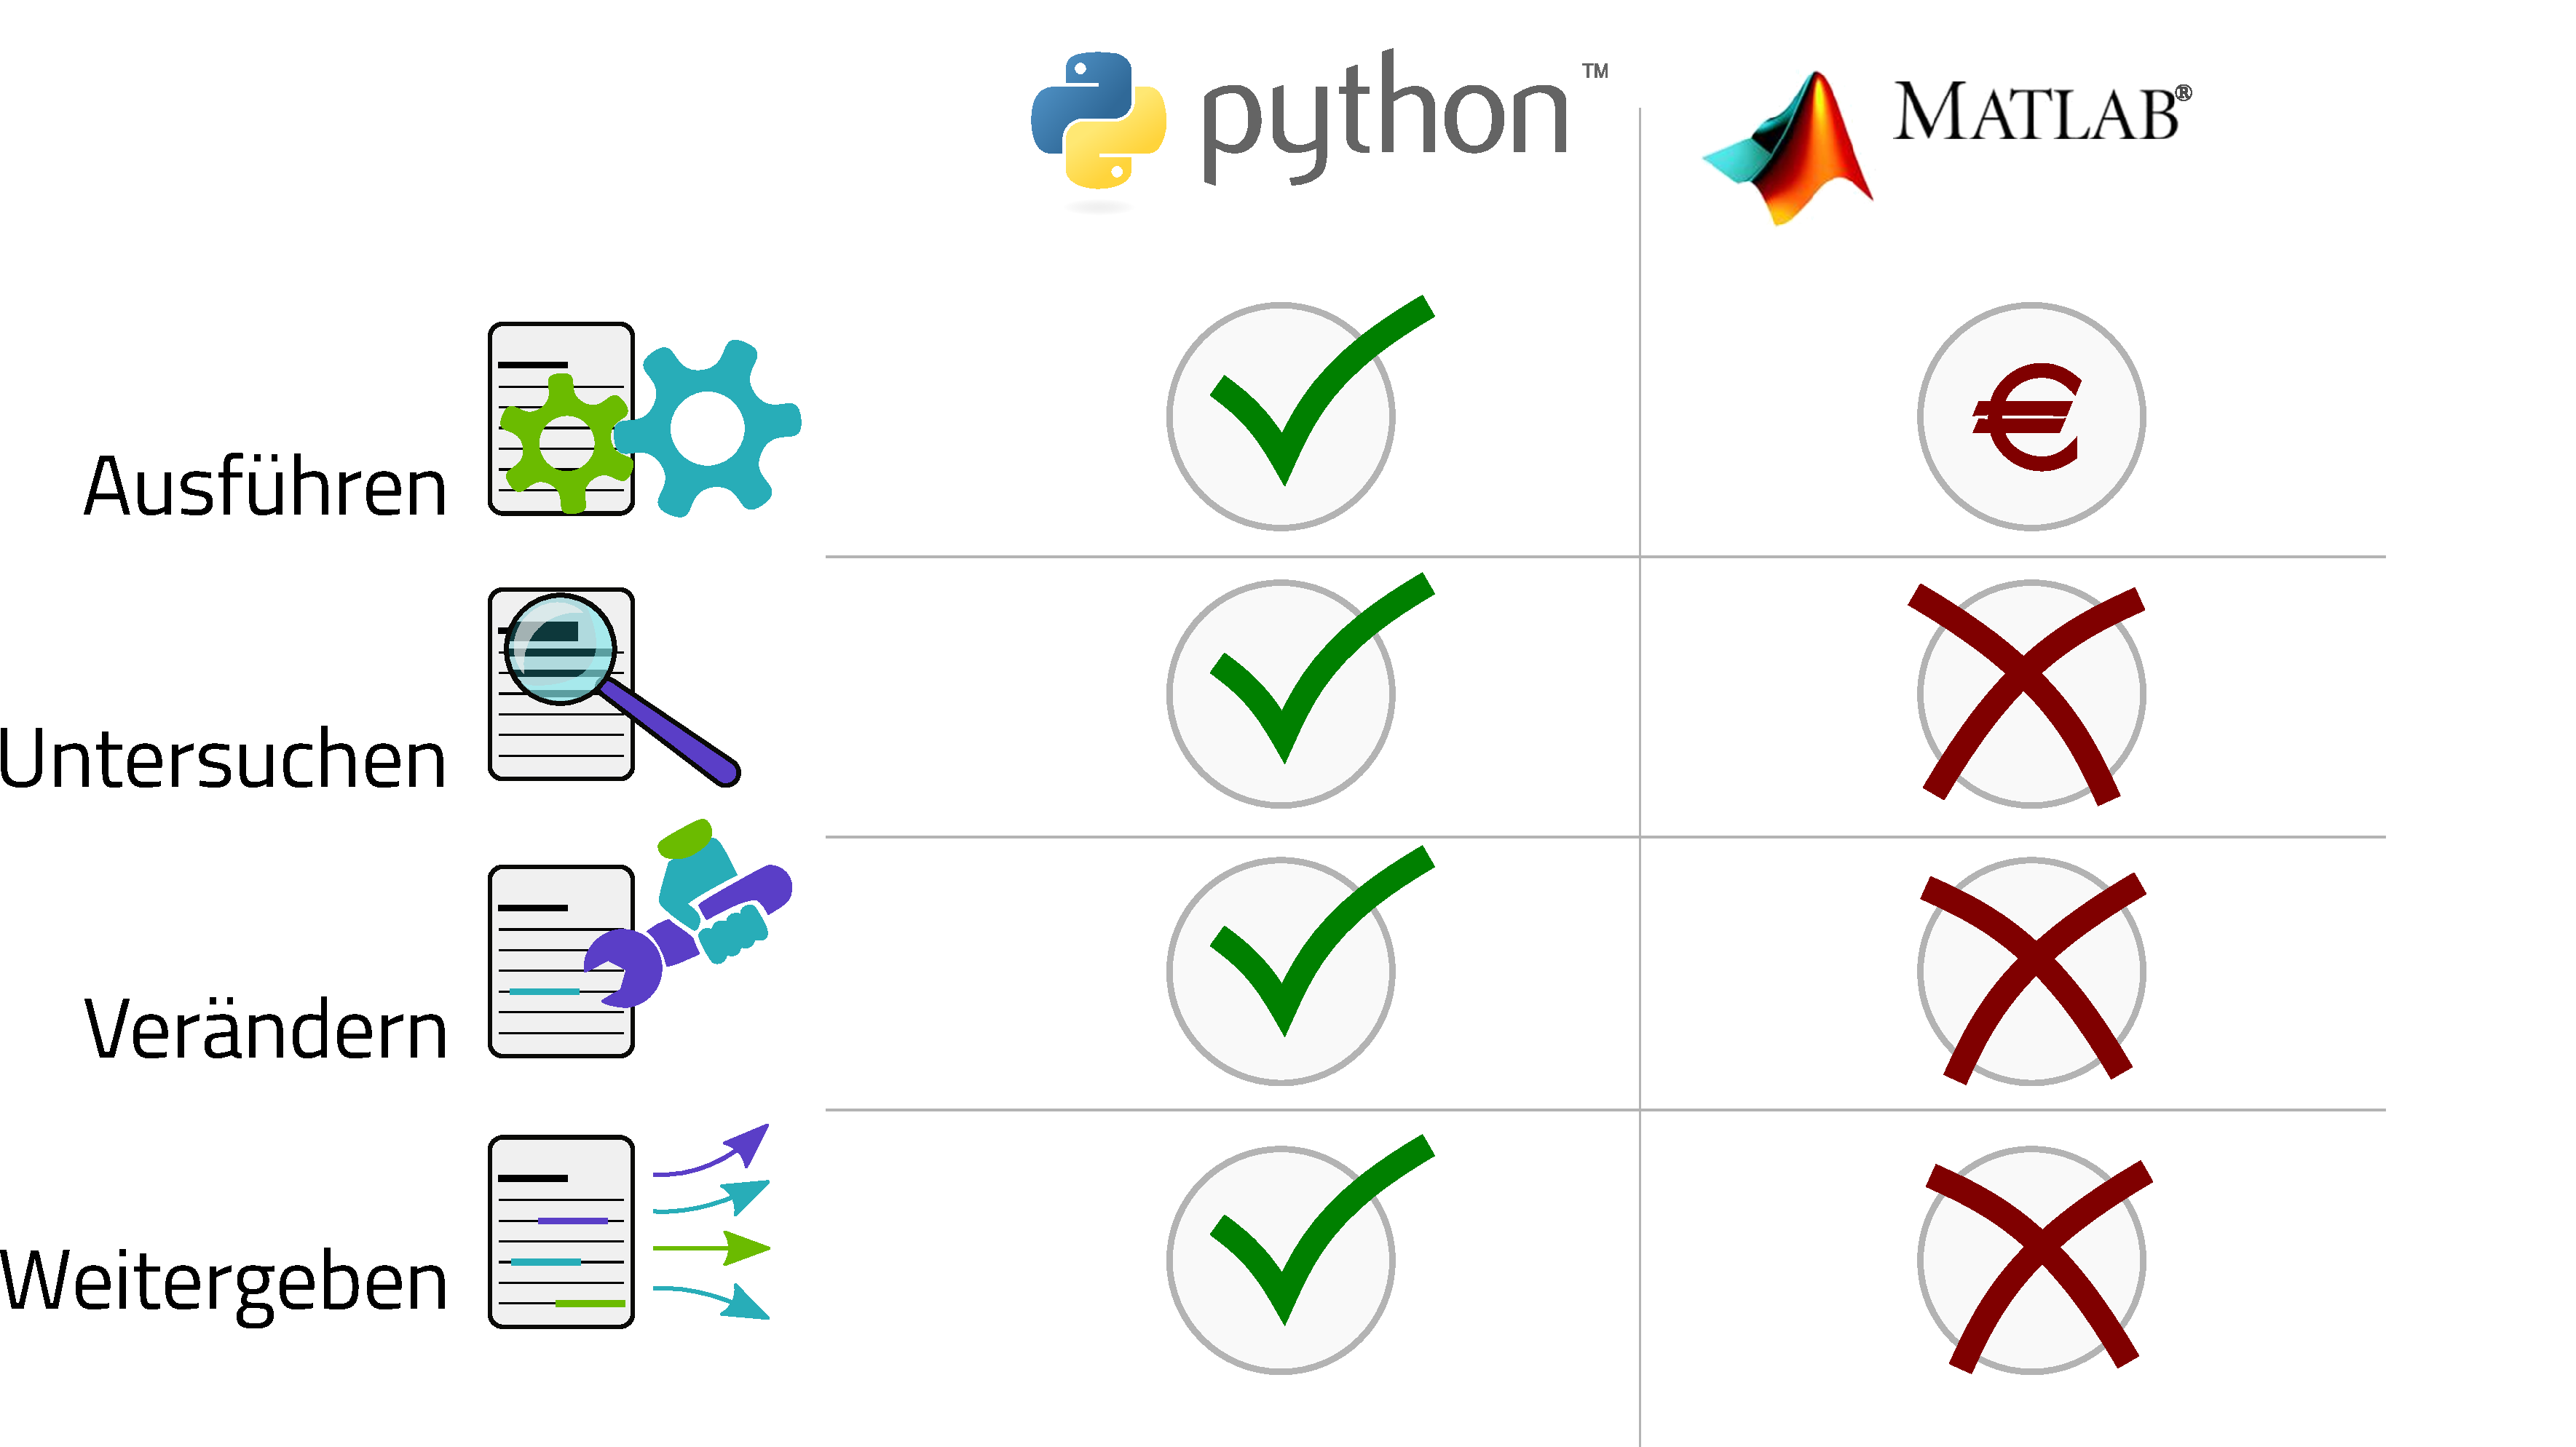
\includegraphics[width=\textwidth]{img-src/vier-freiheiten-tabelle07}}
\only<8>{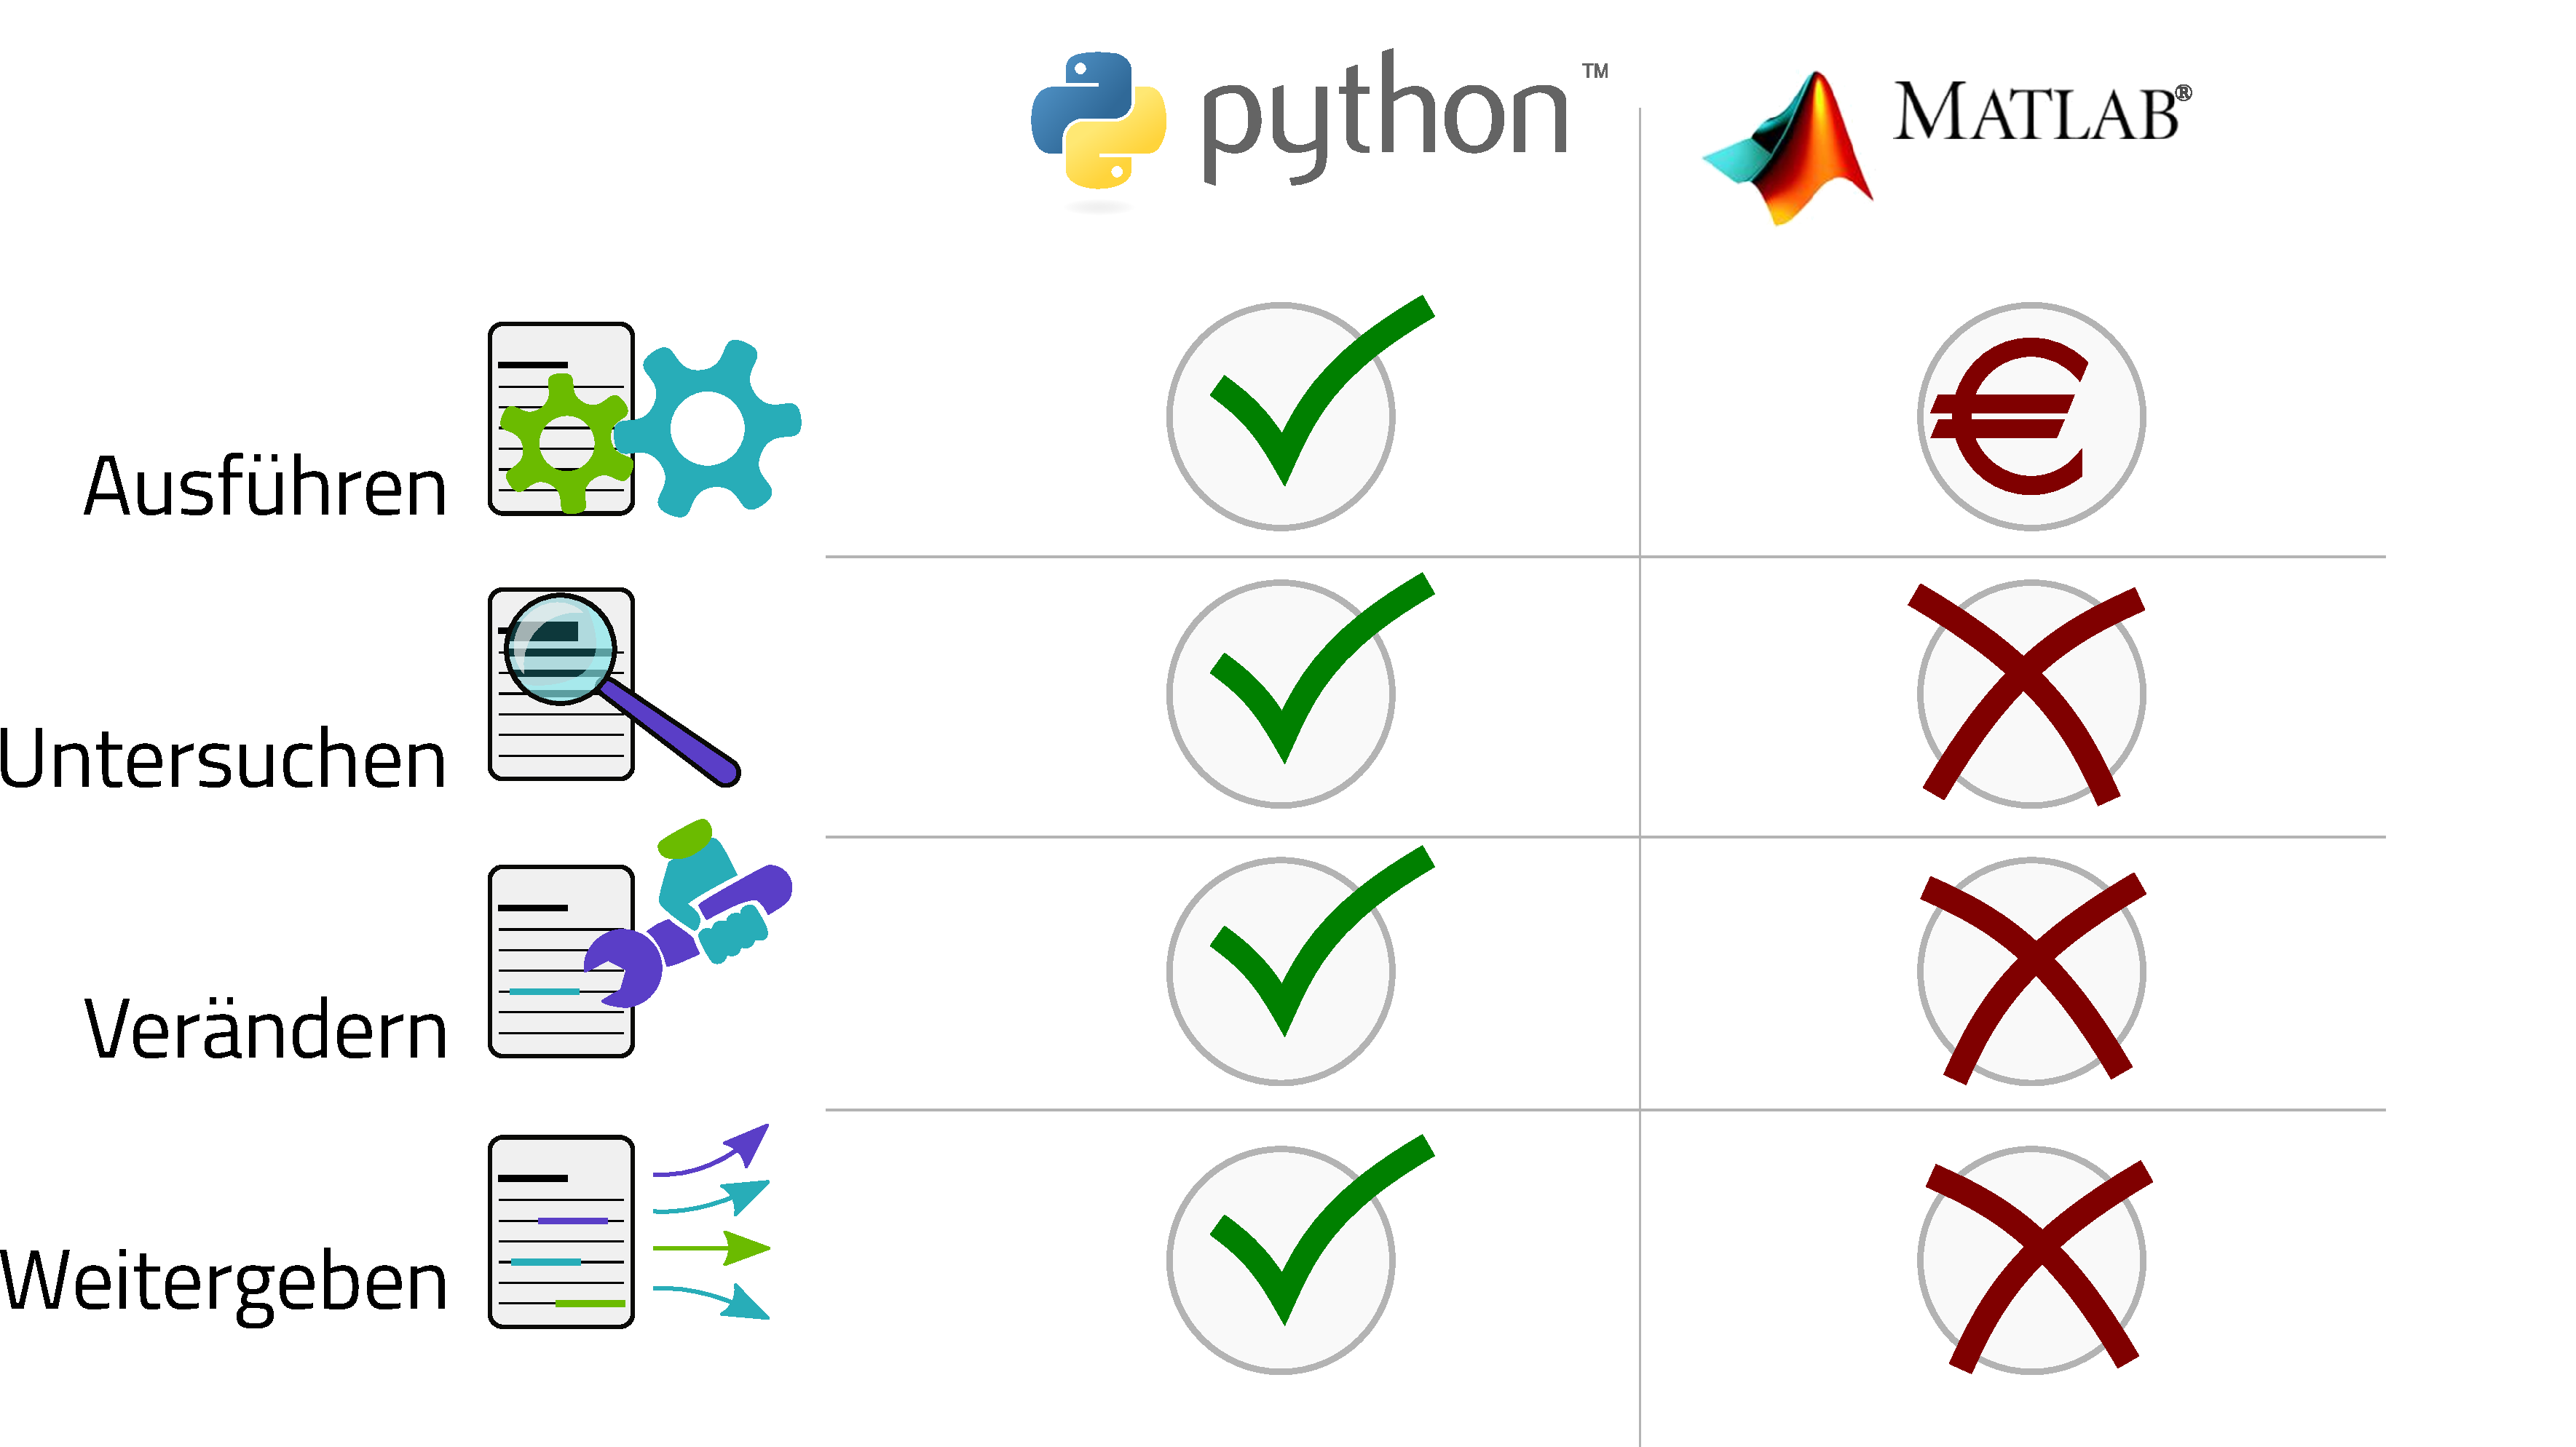
\includegraphics[width=\textwidth]{img-src/vier-freiheiten-tabelle08}}
\only<9>{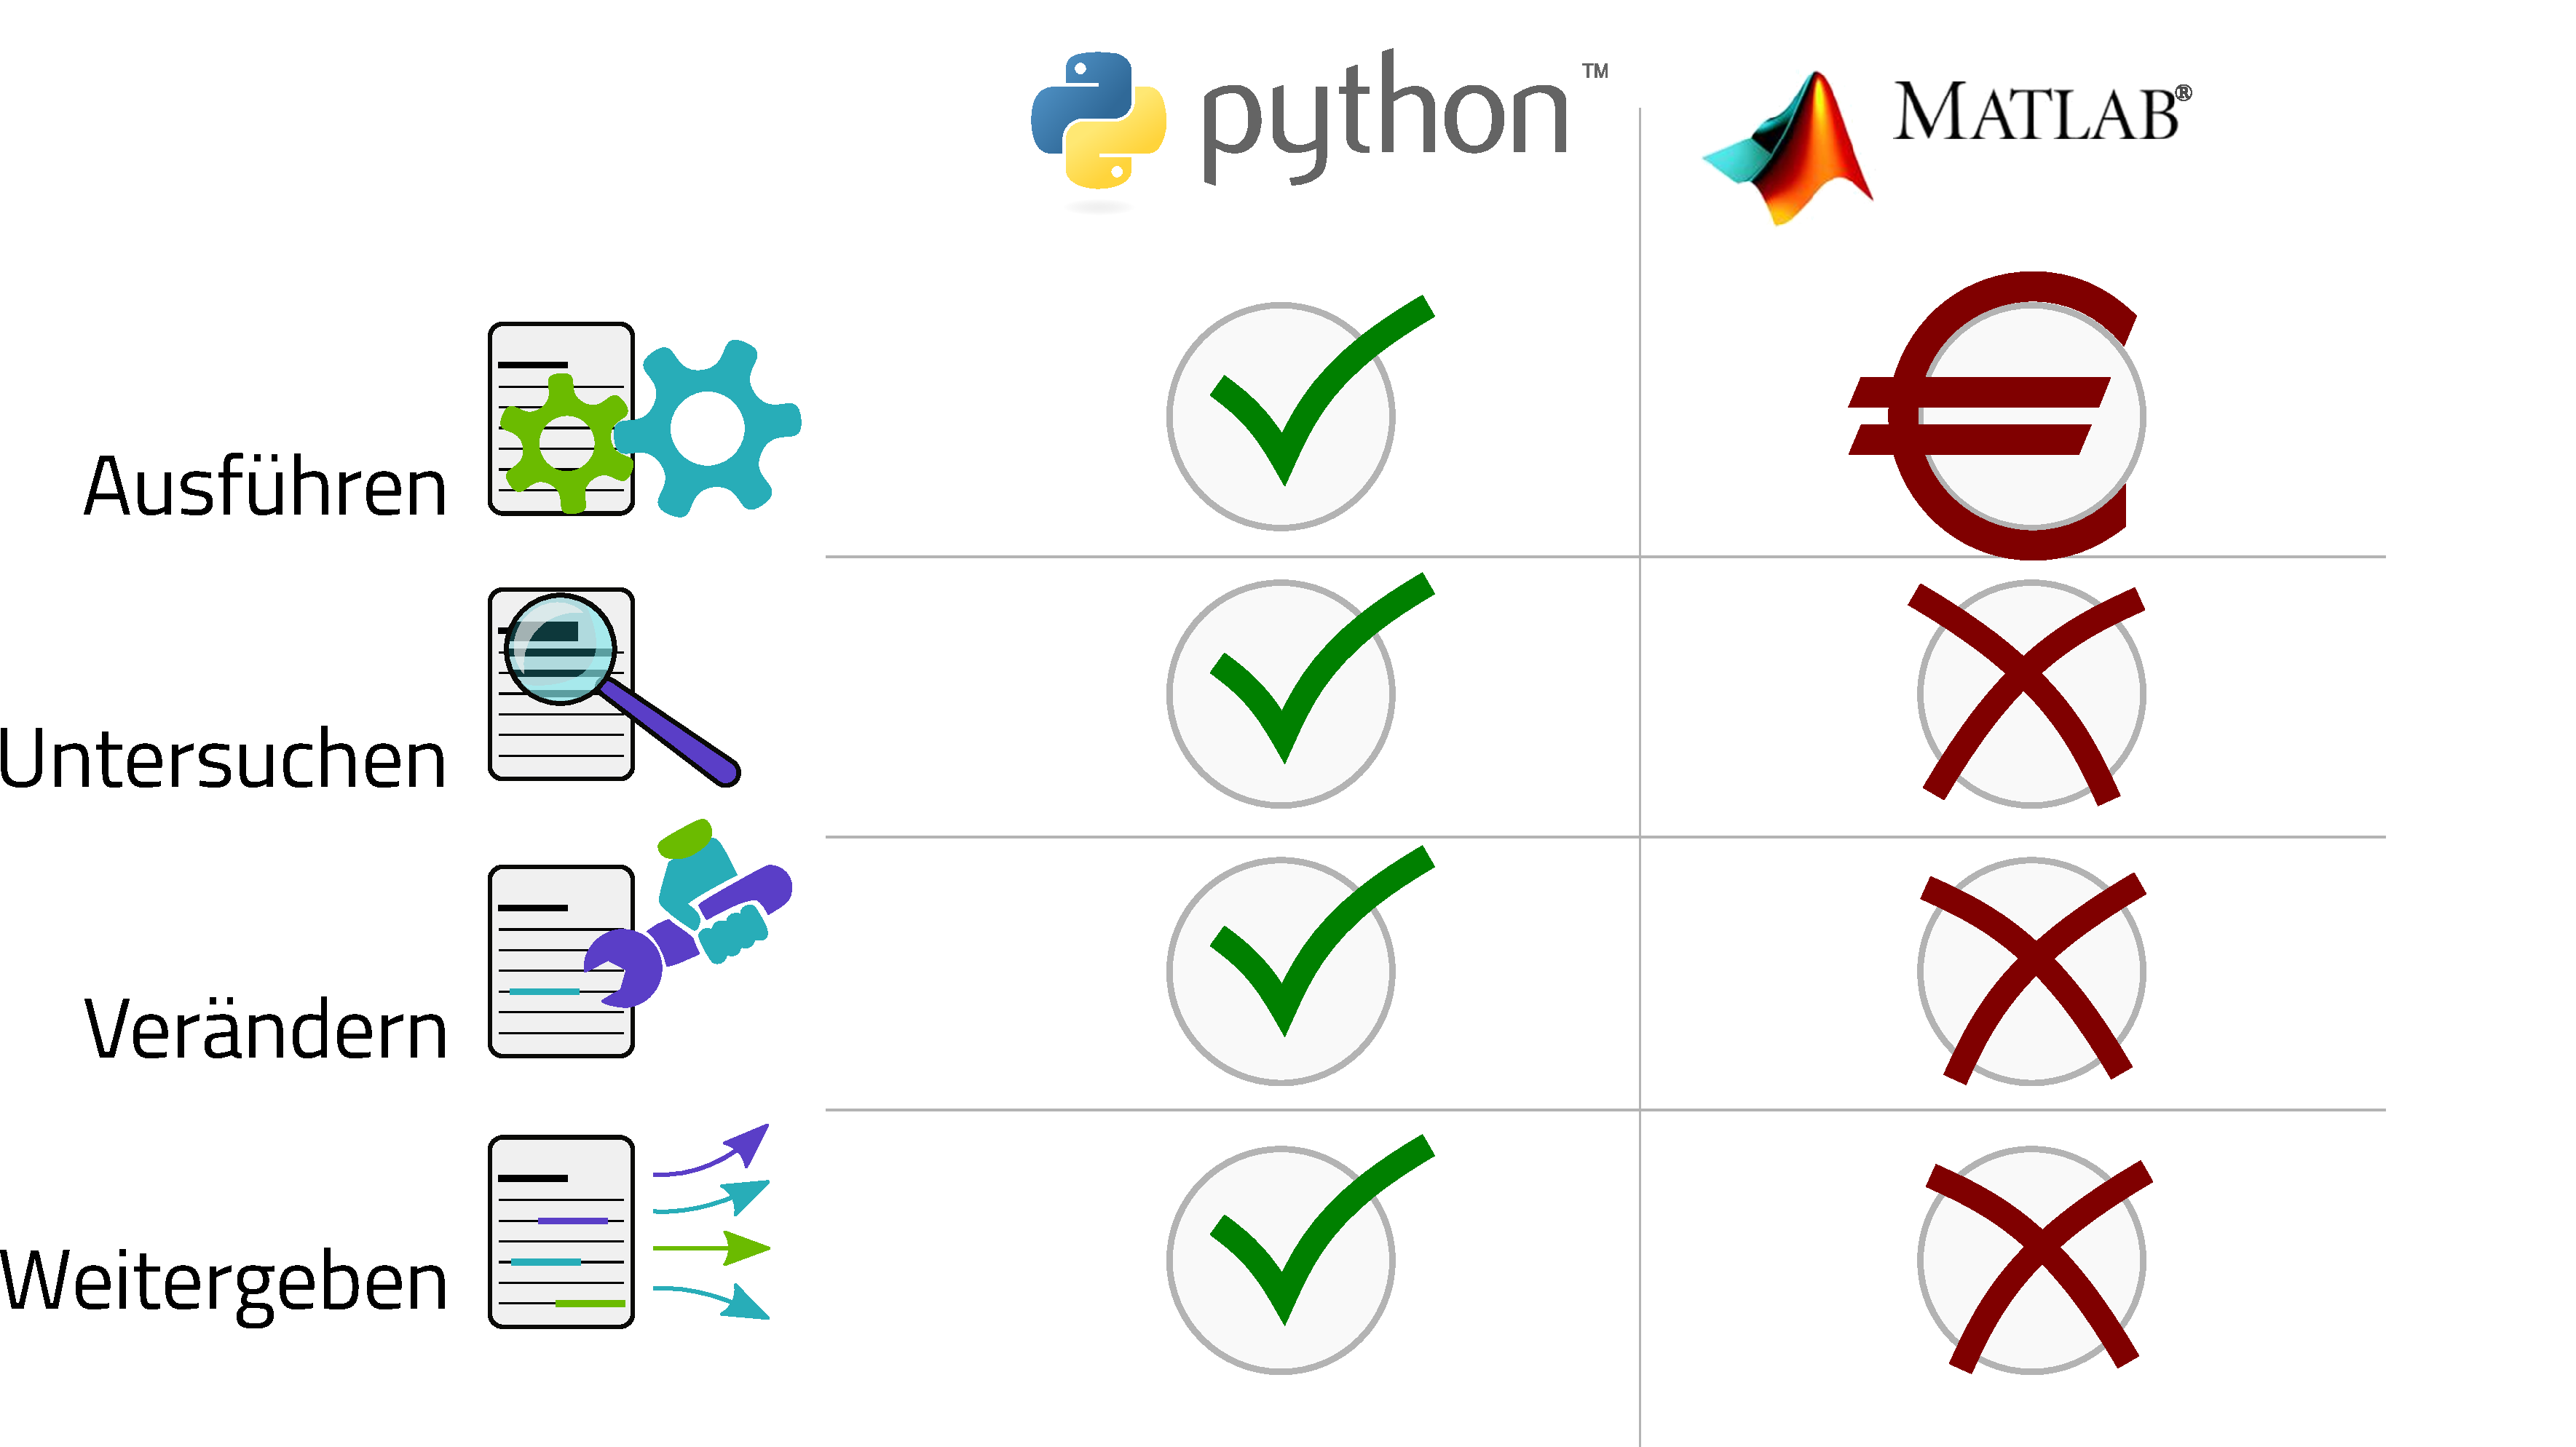
\includegraphics[width=\textwidth]{img-src/vier-freiheiten-tabelle09}}
 
\end{frame}

%%%%%%%%%%%%%%%%%%%%%%%%%%%%%%%%%%%%%%%%%%%%%%%%%%%%%%%%%%%%%%%%%%%%%%%%%%%%%%%%

\begin{frame}[label=ct1]{\usebeamercolor[fg]{structure}\color{fg}Was tut die FSFW? }
  \begin{itemize}
   \item Linux: Install-Party, Presentation-Day
   \item Verschlüsselungsgewinnspiel
   \item Monatliche {Sprechstunde} (\LaTeX, Linux, ...)
%    \item Programmpapier (Lobbyismus)
   \item Workshops (\raisebox{-.3em}{
\includegraphics[height=1em]{img-src/Git-Logo-2Color}}, Mailverschlüsselung)
   \item Uni-Stick mit freier Software $\rightarrow$ Erstitüten
  \end{itemize}
  \begin{center}
   \pause
   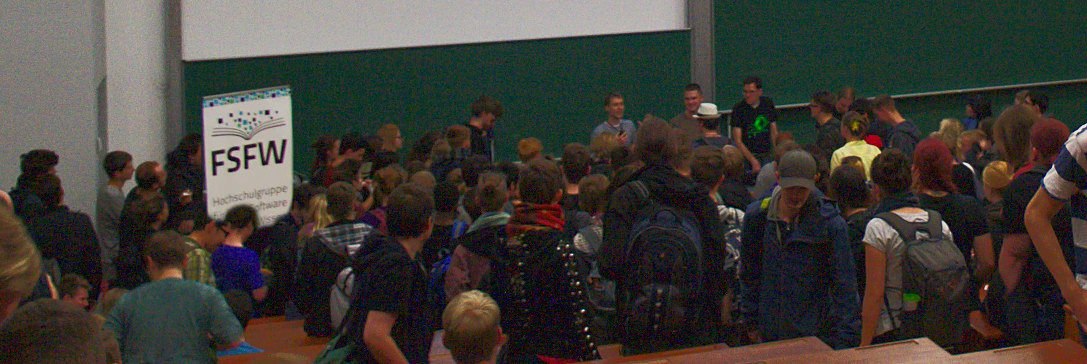
\includegraphics[width=70mm]{img-src/stick-ausgabe-2017}
  \end{center}
\end{frame}

%%%%%%%%%%%%%%%%%%%%%%%%%%%%%%%%%%%%%%%%%%%%%%%%%%%%%%%%%%%%%%%%%%%%%%%%%%%%%%%%


\begin{frame}[label=ct5]{\usebeamercolor[fg]{structure}\color{fg}{}}
 \vspace{6mm}


\begin{columns}
\column[t]{0.9\textwidth}

\begin{flushright}
\huge
\url{fsfw-dresden.de/mitmachen}\\
{\tiny Plenum: Do. (ungerade KW, SLUB)}\\[3mm]
\end{flushright}
\column[t]{0.1\textwidth}
~
\end{columns}

 
  \begin{textblock*}{55mm}[0.,0.5](35mm,60.6mm)
  \visible<2->{
 
\includegraphics[width=50mm]{img-src/fsfw-netzwerke}
}
 \end{textblock*}




% \end{center}
\end{frame}


%%%%%%%%%%%%%%%%%%%%%%%%%%%%%%%%%%%%%%%%%%%%%%%%%%%%%%%%%%%%%%%%%%%%%%%%%%%%%%%%


% 
% \begin{frame}[label=wb]{\usebeamercolor[fg]{structure}\color{fg} Vier (Un)Freiheiten}
% 
% \begin{columns}
% 
% \column[t]{0.02\textwidth}
% 
% ~
% \column[t]{0.5\textwidth}
% 
% 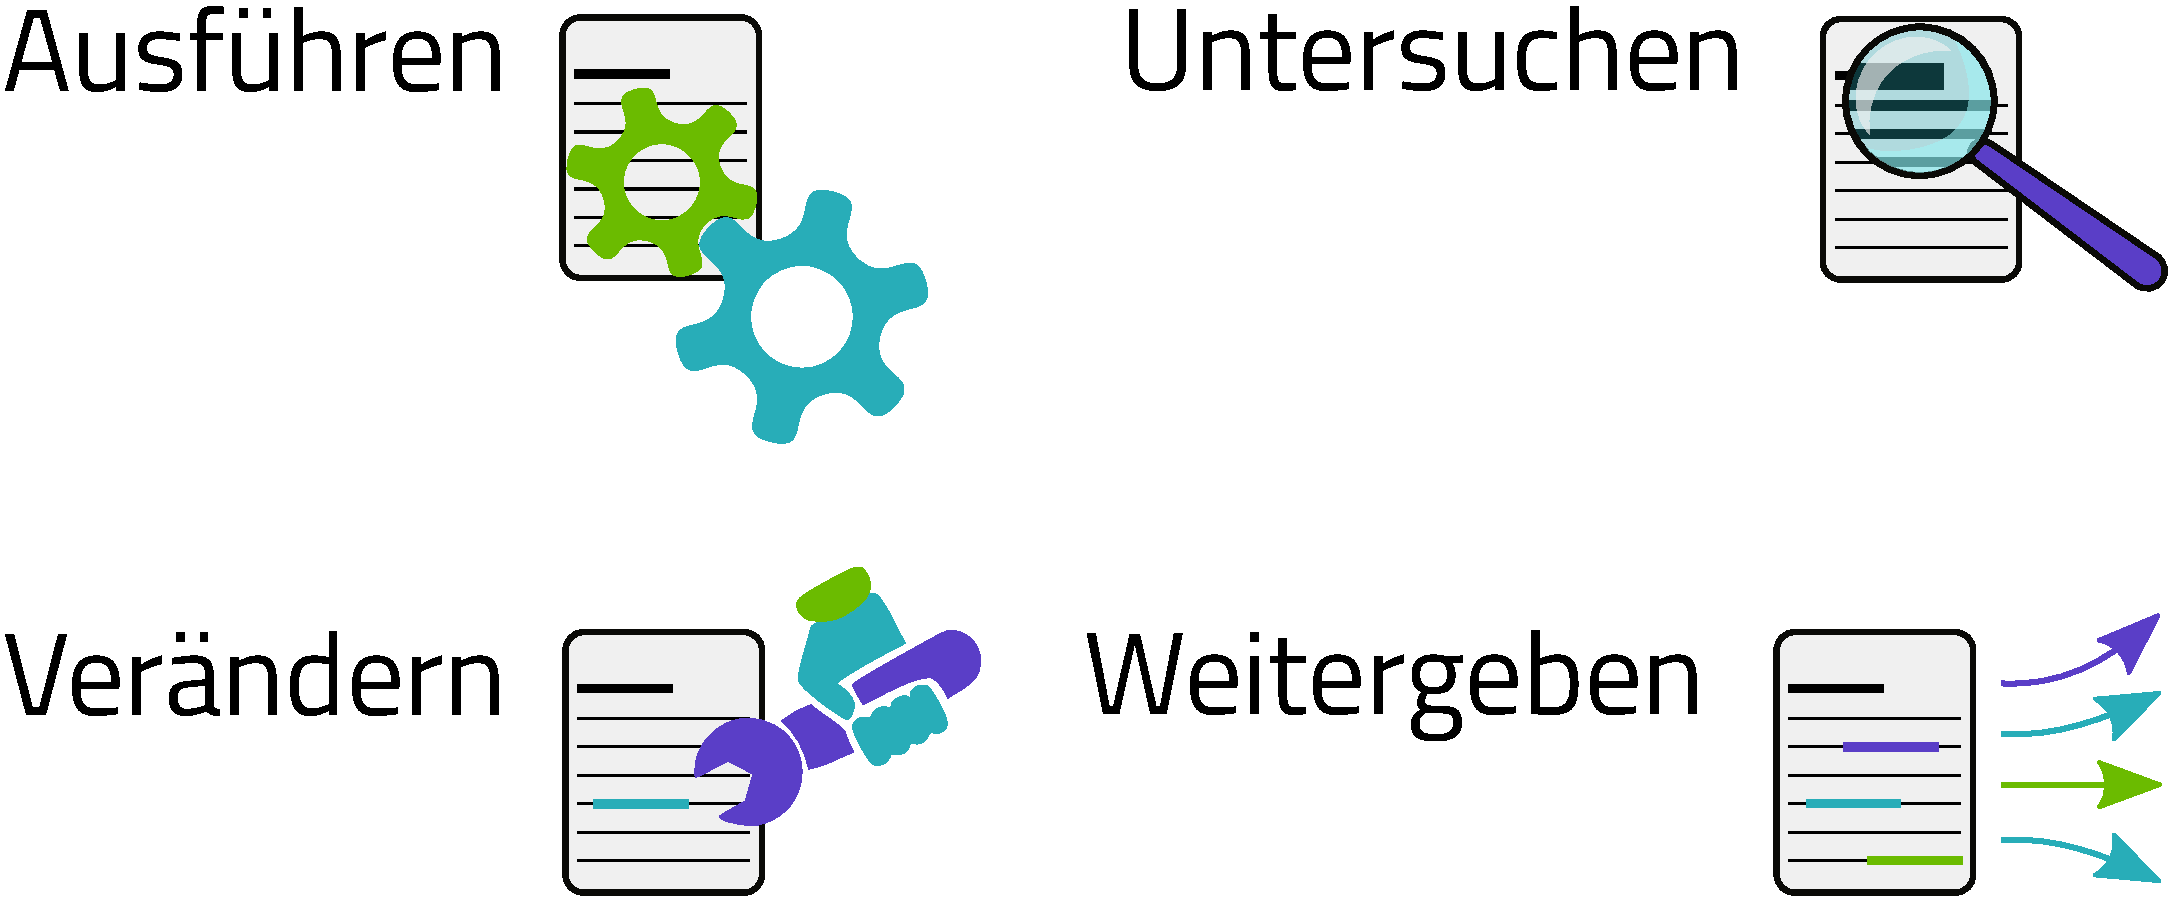
\includegraphics[width=40mm]{img-src/vier-freiheiten}
% \pause
% 
% Vorteile:
% \begin{itemize}
% \item Kontrolle behalten
% \item Erkenntnisgewinn
% \item Lizenzkosten: 0 €
% \item Anpassbarkeit an eigene Bedürfnisse
% \item Hersteller-Unabhängigkeit\\[-2mm] {\tiny (kein Vendor Lock-in)}
% 
% \end{itemize}
% 
% 
% \column[t]{0.01\textwidth}
% ~
% \column[t]{0.58\textwidth}
% Nachteile Proprietärer Software
% \begin{itemize}
%  \item Intransparenz {\tiny (Bsp: Wahlsoftware)}
%  \item Hintertüren? {\tiny (Win10-Verbot für Dienstgebrauch)}
%  \item Abhängigkeit
% \end{itemize}
%  \pause
%  \bigskip
% 
% 
%  \textit{Warum gibt es MS-Office eigentlich {\color<4->{red} \visible<4->{"`}kostenlos\visible<4->{"'}} für Studierende?}
% 
%  \pause
%  \pause
%  \medskip
%  \rule{\textwidth}{1pt}\\[2mm]
% %  \smallskip
%  Offener Brief:\\
% 
%  "`public money $\Rightarrow$ public code"'\\[2mm]
% 
%  \url{https://publiccode.eu}
% 
% 
% \end{columns}
% 
% \end{frame}



%%%%%%%%%%%%%%%%%%%%%%%%%%%%%%%%%%%%%%%%%%%%%%%%%%%%%%%%%%%%%%%%%%%%%%%%%%%%%%%%


% 
% \begin{frame}{\usebeamercolor[fg]{structure}\color{fg}Arbeitsthesen}
%   \begin{itemize}
%   \item<1-> Freie Software und freies Wissen fördert die Bildung einer aufgeklärten digitalen Gesellschaft
%   \item<2-> Freie Software fördert Wahlfreiheit und schützt vor Abhängigkeit
%   \item<3-> Freie Software erhöht Nachvollziehbarkeit
%   \item<4-> Freie Lizenzen sichern den ungehinderten Zugang zu öffentlich finanzierter Forschung
%   \end{itemize}
% \end{frame}

\end{document}
